\documentclass[]{book}
\usepackage{lmodern}
\usepackage{amssymb,amsmath}
\usepackage{ifxetex,ifluatex}
\usepackage{fixltx2e} % provides \textsubscript
\ifnum 0\ifxetex 1\fi\ifluatex 1\fi=0 % if pdftex
  \usepackage[T1]{fontenc}
  \usepackage[utf8]{inputenc}
\else % if luatex or xelatex
  \ifxetex
    \usepackage{mathspec}
  \else
    \usepackage{fontspec}
  \fi
  \defaultfontfeatures{Ligatures=TeX,Scale=MatchLowercase}
\fi
% use upquote if available, for straight quotes in verbatim environments
\IfFileExists{upquote.sty}{\usepackage{upquote}}{}
% use microtype if available
\IfFileExists{microtype.sty}{%
\usepackage{microtype}
\UseMicrotypeSet[protrusion]{basicmath} % disable protrusion for tt fonts
}{}
\usepackage[margin=1in]{geometry}
\usepackage{hyperref}
\hypersetup{unicode=true,
            pdftitle={R: Uma Introdução para economistas},
            pdfauthor={Daniel Coutinho},
            pdfborder={0 0 0},
            breaklinks=true}
\urlstyle{same}  % don't use monospace font for urls
\usepackage{natbib}
\bibliographystyle{apalike}
\usepackage{color}
\usepackage{fancyvrb}
\newcommand{\VerbBar}{|}
\newcommand{\VERB}{\Verb[commandchars=\\\{\}]}
\DefineVerbatimEnvironment{Highlighting}{Verbatim}{commandchars=\\\{\}}
% Add ',fontsize=\small' for more characters per line
\usepackage{framed}
\definecolor{shadecolor}{RGB}{248,248,248}
\newenvironment{Shaded}{\begin{snugshade}}{\end{snugshade}}
\newcommand{\KeywordTok}[1]{\textcolor[rgb]{0.13,0.29,0.53}{\textbf{#1}}}
\newcommand{\DataTypeTok}[1]{\textcolor[rgb]{0.13,0.29,0.53}{#1}}
\newcommand{\DecValTok}[1]{\textcolor[rgb]{0.00,0.00,0.81}{#1}}
\newcommand{\BaseNTok}[1]{\textcolor[rgb]{0.00,0.00,0.81}{#1}}
\newcommand{\FloatTok}[1]{\textcolor[rgb]{0.00,0.00,0.81}{#1}}
\newcommand{\ConstantTok}[1]{\textcolor[rgb]{0.00,0.00,0.00}{#1}}
\newcommand{\CharTok}[1]{\textcolor[rgb]{0.31,0.60,0.02}{#1}}
\newcommand{\SpecialCharTok}[1]{\textcolor[rgb]{0.00,0.00,0.00}{#1}}
\newcommand{\StringTok}[1]{\textcolor[rgb]{0.31,0.60,0.02}{#1}}
\newcommand{\VerbatimStringTok}[1]{\textcolor[rgb]{0.31,0.60,0.02}{#1}}
\newcommand{\SpecialStringTok}[1]{\textcolor[rgb]{0.31,0.60,0.02}{#1}}
\newcommand{\ImportTok}[1]{#1}
\newcommand{\CommentTok}[1]{\textcolor[rgb]{0.56,0.35,0.01}{\textit{#1}}}
\newcommand{\DocumentationTok}[1]{\textcolor[rgb]{0.56,0.35,0.01}{\textbf{\textit{#1}}}}
\newcommand{\AnnotationTok}[1]{\textcolor[rgb]{0.56,0.35,0.01}{\textbf{\textit{#1}}}}
\newcommand{\CommentVarTok}[1]{\textcolor[rgb]{0.56,0.35,0.01}{\textbf{\textit{#1}}}}
\newcommand{\OtherTok}[1]{\textcolor[rgb]{0.56,0.35,0.01}{#1}}
\newcommand{\FunctionTok}[1]{\textcolor[rgb]{0.00,0.00,0.00}{#1}}
\newcommand{\VariableTok}[1]{\textcolor[rgb]{0.00,0.00,0.00}{#1}}
\newcommand{\ControlFlowTok}[1]{\textcolor[rgb]{0.13,0.29,0.53}{\textbf{#1}}}
\newcommand{\OperatorTok}[1]{\textcolor[rgb]{0.81,0.36,0.00}{\textbf{#1}}}
\newcommand{\BuiltInTok}[1]{#1}
\newcommand{\ExtensionTok}[1]{#1}
\newcommand{\PreprocessorTok}[1]{\textcolor[rgb]{0.56,0.35,0.01}{\textit{#1}}}
\newcommand{\AttributeTok}[1]{\textcolor[rgb]{0.77,0.63,0.00}{#1}}
\newcommand{\RegionMarkerTok}[1]{#1}
\newcommand{\InformationTok}[1]{\textcolor[rgb]{0.56,0.35,0.01}{\textbf{\textit{#1}}}}
\newcommand{\WarningTok}[1]{\textcolor[rgb]{0.56,0.35,0.01}{\textbf{\textit{#1}}}}
\newcommand{\AlertTok}[1]{\textcolor[rgb]{0.94,0.16,0.16}{#1}}
\newcommand{\ErrorTok}[1]{\textcolor[rgb]{0.64,0.00,0.00}{\textbf{#1}}}
\newcommand{\NormalTok}[1]{#1}
\usepackage{longtable,booktabs}
\usepackage{graphicx,grffile}
\makeatletter
\def\maxwidth{\ifdim\Gin@nat@width>\linewidth\linewidth\else\Gin@nat@width\fi}
\def\maxheight{\ifdim\Gin@nat@height>\textheight\textheight\else\Gin@nat@height\fi}
\makeatother
% Scale images if necessary, so that they will not overflow the page
% margins by default, and it is still possible to overwrite the defaults
% using explicit options in \includegraphics[width, height, ...]{}
\setkeys{Gin}{width=\maxwidth,height=\maxheight,keepaspectratio}
\IfFileExists{parskip.sty}{%
\usepackage{parskip}
}{% else
\setlength{\parindent}{0pt}
\setlength{\parskip}{6pt plus 2pt minus 1pt}
}
\setlength{\emergencystretch}{3em}  % prevent overfull lines
\providecommand{\tightlist}{%
  \setlength{\itemsep}{0pt}\setlength{\parskip}{0pt}}
\setcounter{secnumdepth}{5}
% Redefines (sub)paragraphs to behave more like sections
\ifx\paragraph\undefined\else
\let\oldparagraph\paragraph
\renewcommand{\paragraph}[1]{\oldparagraph{#1}\mbox{}}
\fi
\ifx\subparagraph\undefined\else
\let\oldsubparagraph\subparagraph
\renewcommand{\subparagraph}[1]{\oldsubparagraph{#1}\mbox{}}
\fi

%%% Use protect on footnotes to avoid problems with footnotes in titles
\let\rmarkdownfootnote\footnote%
\def\footnote{\protect\rmarkdownfootnote}

%%% Change title format to be more compact
\usepackage{titling}

% Create subtitle command for use in maketitle
\newcommand{\subtitle}[1]{
  \posttitle{
    \begin{center}\large#1\end{center}
    }
}

\setlength{\droptitle}{-2em}

  \title{R: Uma Introdução para economistas}
    \pretitle{\vspace{\droptitle}\centering\huge}
  \posttitle{\par}
    \author{Daniel Coutinho}
    \preauthor{\centering\large\emph}
  \postauthor{\par}
      \predate{\centering\large\emph}
  \postdate{\par}
    \date{Última Atualização: 17/10/2018}


\begin{document}
\maketitle

{
\setcounter{tocdepth}{1}
\tableofcontents
}
\chapter{Introdução}\label{introducao}

Existem muitos softwares de estatística, mas o R é um dos mais
populares. O R é um software gratuito, o que justifica a sua escolha.
Mas além disso, a comunidade é muito ativa, desenvolvendo muitos pacotes
- inclusive para econometria. O R não é tão amigável quanto o gretl: não
existem menus para escolher como estimar. Entretanto, ele é muito mais
flexível. Assim, o R tem ganho cada vez mais espaço entre aqueles que
fazem econometria.

Este manual foi criado para ajudar a introduzir economistas ao R. Com
isso, ele é mais voltado para exemplos de tratamento de dados e
ferramentas estatísticas usadas pelos economistas. Existem outros
excelentes livros que ensinam a usar o R, e alguns aplicados à
econometria. Eles estão listados nas referências deste manual. Mas
nenhum deles é em português, e muitos são muito detalhistas e longos.
Este manual tenta servir como algo menos extenso que os livros.
Portanto, uma consulta aos livros pode ser muito útil.

Esta é a segunda versão do manual, que foi extensivamente reescrito em
meados de 2017 e início de 2018. Não é necessário nenhuma experiência
anterior com programação, mas é necessário saber (alguma) econometria. O
autor agradece as muitas pessoas na PUC-Rio que ajudaram com o R, bem
como os seis meses trabalhando no Dlab. As duas versões anteriores foram
escritas, originalmente, em LaTeX, o \emph{gold standard} da edição de
texto acadêmica.Essa versão foi escrita usando o bookdown, um pacote do
R para produzir livros para a internet.

Algumas palavras sobre a filosofia por trás desse manual são
necessárias: a ideia é tirar o leitor do chão e colocar ele pronto para
fazer as coisas básicas de econometria rapidamente. Isso envolve
notórias omissões. O autor muitas vezes sugere consultar o help, o que
deve ser visto não como preguiça, mas sim como a única maneira de fazer
as coisas: existem mais de 12 mil pacotes disponíveis para o R, e nenhum
ser humano jamais conseguirá explorar e entender todos. O autor usou,
diretamente, uma dúzia pacotes, se tanto. E invariavelmente é necessário
consultar o help para saber qual o nome do argumento que faz alguma
coisa específica. Assim, a ideia aqui é entender as ideias gerais do R,
os comandos básicos e o mínimo do vocabulário para saber consultar/ler o
help.

Definitivamente esse manual deve ser lido com o R aberto e tentando
entender cada um dos comandos que são ditos aqui. Uma leitura
comparativa entre o help e o que eu coloco no manual sobre cada comando
é provavelmente a melhor maneira de proceder. Tentar replicar tudo que
eu faço é uma maneira garantida de aprender. As seções Hands on propõe
exercícios específicos para serem feitos no R. O capítulo projetinhos
tem o mesmo objetivo, mas com exercícios que são mais extensos.

O manual é dividido em três partes: a primeira trata de como fazer
econometria no R: é o coração do manual e é de principal interesse dos
economistas; a segunda parte trata de como programar no R, o que é útil
em algumas atividades um pouco mais avançadas. A terceira parte será
dedicada a algumas coisas de matemática no R. Seções marcadas com um *
são mais indigestas para a primeira leitura.

\chapter{Primeiros Passos}\label{primeiros-passos}

\section{Instalação}\label{instalacao}

\subsection{Instalando o R e o
RStudio}\label{instalando-o-r-e-o-rstudio}

Instalar o R é trivial: basta ir no \url{http://cran.r-project.org/} e
baixar a versão para o seu computador. Exceto se você usar alguma
distribuição de Linux (Ubuntu, por exemplo): ai é mais difícil, mas o
próprio CRAN dá instruções de como fazer. Depois, recomenda-se baixar o
R Studio, disponível em \url{https://www.rstudio.org/}. O R Studio é uma
IDE (Integrated Development Enviroment), que facilita muito a vida na
hora de programar - especialmente dando sugestões de comandos e
mostrando quais variáveis estão salvas no ambiente do R. Assim, sugiro
instalar o R Studio, que é bem tranquilo. Para usar o R Studio, você
precisa ter o R.

\subsection{Uma alternativa}\label{uma-alternativa}

Se o seu computador tem um processador multi-core, pode ser interessante
instalar o Microsoft R, disponível em \url{http://mran.microsoft.com/}.
Ele é idêntico ao R, mas vem com uma biblioteca que tira vantagem dos
vários núcleos do processador, o que o R padrão não faz. A principal
desvantagem é que ele é atualizado com menos frequência, e a biblioteca
que usa mais de um núcleo não está disponível para o Mac. Ele funciona
com o R Studio.

\subsection{Interface}\label{interface}

A interface do R Studio mostra 4 espaços diferentes: no canto esquerdo
superior, existe uma tela chamada source (se ela não estiver lá, tente
usar ctrl + shift + n para abrir); a direita dela, o ambiente; no canto
inferior esquerdo, está o console; e no canto inferior direito está uma
tela multiuso, que deve vir com as abas plot, files. Cada uma dessas
será explicada, por alto, nesta seção

A que mais nos interessa, em um primeiro momento, é o console. Nele,
você pode passar comandos direto para o R. Digitando 2 + 2 nele e
clicando em enter, o resultado deve aparecer na tela. Em geral, é nele
que você vai trabalhar. Entretanto, escrever código muito longos no
console é muito ruim. O console é desorganizado, não permite salvar o
código passado para ele para ser usado mais tarde e não permite com que
você corrija erros com facilidade. O source serve justamente para
escrever um código longo - uma função ou uma simulação, por exemplo -
que pode ser executado no console. Para isso, basta selecionar o
conteúdo e dar ctrl + enter ou chegar no fim da linha e usar ctrl +
enter.

A tela do canto direito inferior é uma ``geleia geral'': a aba plots é
onde os gráficos que faremos vão aparecer; a aba files permite você ver
arquivos em diferentes pastas do computador. Estas são as abas mais
importantes e que mais serão usadas. Em cima desta tela, há a tela
\emph{environment}, que mostra as variáveis que foram criadas e estão
disponíveis para o R usar

\section{Erros, Warnings e letras
vermelhas}\label{erros-warnings-e-letras-vermelhas}

Tão importante quanto saber fazer a coisa certa é saber quando temos um
problema. Existem dois tipos de erro:

\begin{itemize}
\tightlist
\item
  Error: esses são de fato erros, e o R não consegue proceder. O que
  você escreveu tem algum problema grave e não pode ser executado.
\item
  Warning: o R conseguiu fazer o que você pediu, mas alguma coisa
  esquisita aconteceu, e o R está te avisando.
\end{itemize}

Veja que em ambos os casos a mensagem vai aparecer em vermelho no
console. \emph{Error} e \emph{warnings} vem das mais diferentes formas
(afinal, é possível errar de diferentes formas). Alguns são claros, como
tentar somar um número e uma letra:

\begin{Shaded}
\begin{Highlighting}[]
\DecValTok{2} \OperatorTok{+}\StringTok{ "a"}
\end{Highlighting}
\end{Shaded}

\begin{verbatim}
## Error in 2 + "a": argumento não-numérico para operador binário
\end{verbatim}

(Apesar de operador binário não ser exatamente óbvio)

Outros são mais misteriosos, e quando encontramos um erro impossível de
entender, coloque o \emph{output} do console no google. Typos geram
muitos erros (ex.: esquecer o parêntese, errar o nome de um objeto). Em
um código longo, descobrir o erro pode ser difícil. Existem ferramentas
para isso, e o próprio \emph{source} do RStudio indica linhas com algum
erro com um x vermelho do lado do número da linha. Em geral, em um
código muito longo, não é uma estratégia ruim escrever uma parte do
código, testar e debugar (retirar os erros) ela. Funções ajudam a fazer
isso: trataremos delas mais a frente.

É importante notar que, apesar de uma linha de código que devolva um
\emph{warning} não está errada, ela pode muito bem fazer uma coisa que
você não quer. Assim, um warning surpresa deve ser visto com bastante
cuidado e normalmente você não deve ignorar um warning.

Veja que essas mensagens não são as únicas que aparecem em vermelho no
R: quando o R instala ou carrega um pacote ele exibe algumas coisas em
vermelho\footnote{Letras em vermelho ocorrem em algumas outras
  situações.}. Não se preocupe: isso não quer dizer que o R encontrou
algum erro ou warning ao instalar o pacote, é apenas o comportamento
padrão do R.

\subsection{Pacotes}\label{pacotes}

O grande atrativo do R são os pacotes. Para instalar um pacote, basta
digitar no console:

\begin{verbatim}
install.packages("nome-do-pacote")
\end{verbatim}

É necessário colocar as aspas para o pacote instalar. Uma vez instalado,
o pacote não é carregado automaticamente. Para carregar o pacote, basta
digitar no console:

\begin{verbatim}
library(nome-do-pacote)
\end{verbatim}

Agora as aspas não são necessárias.

Instalar pacote por pacote pode ser uma tarefa chata. Além do mais, isto
exige que você saiba quais são os pacotes que fazem cada coisa.
Felizmente, o CRAN mantém coleções de pacotes de determinados temas,
chamados de Task Views. Existe um de econometria, e para instalar ele é
necessário instalar o pacote ctv , e depois o task view de econometria:

\begin{verbatim}
install.packages("ctv")
library(ctv)
install.views("Econometrics")
\end{verbatim}

Como são muitos pacotes, esta operação pode tomar algum tempo. Em geral,
muitos dos pacotes nos task view não são tão úteis, então pode ser
interessante ir no cran, e visitar os task views para selecionar quais
pacotes de lá fazem o que você precisa fazer. Existem vários pacotes,
para diferentes áreas. Para os economistas, além do pacote de
econometria, os pacotes de Time Series, Bayesian, Finance, Machine
Learning podem ser de interesse. De fato, com a expansão das áreas de
pesquisas, muitos outros task views podem ser de interesse! Recomenda-se
visitar o cran para ter uma visão do que está disponível.

Hands on!

Vamos instalar um primeiro pacote que adiciona vários comandos
importantes para econometria e alguns datasets de livros de econometria
(como o Stock Watson). O nome do pacote é AER. Ele vai instalar vários
outros pacotes que ele necessita para funcionar, então a instalação pode
demorar um pouco. Ele será usado de agora por diante, então tenham
certeza que ele está carregado, ou seja, que vocês sempre estão usando o
\texttt{library(AER)} quando abrem o R.

\section{Ajuda}\label{ajuda}

Em 90\% do tempo você vai precisar de olhar o help: seja para lembrar
que opções estão disponíveis em um comando, ou lembrar exatamente o que
o comando faz, ou descobrir qual o comando para fazer alguma coisa
específica que você só tem uma palavra chave: ``Como gera números saídos
de uma distribuição normal mesmo?''\footnote{Dois iguais seguidos}

Se você sabe o comando e quer ler o help deste comando, basta fazer
\texttt{?comando}. Por exemplo, se você quiser saber o que o comando
rnorm faz e quais as opções ele oferece, basta digitar no console
\texttt{?rnorm}. Se você não sabe o nome do comando, mas quer saber
todos os comandos que estão relacionados a uma determinada palavra
chave, use \texttt{??palavra}. Por exemplo, se você quiser saber todos
os comandos que envolvem a distribuição normal, basta usar
\texttt{??normal}. Observe que, se você tiver muitos pacotes, isto pode
demorar um pouco, já que exige que o R procure cada pacote que se
referencie àquela palavra.

Você também pode estar interessado em todos os comandos de um pacote.
Neste caso, a melhor solução é é usar
\texttt{help(package=\textasciigrave{}\textasciigrave{}nome-do-pacote\textquotesingle{}\textquotesingle{})}.

\section{Comentando}\label{comentando}

Em geral, quando se escreve um código, é importante explicar o que
algumas partes do código fazem. Isso não é exclusivo para o caso em que
o código vai ser distribuído: pelo contrário, o você do futuro vai
agradecer muito o você do passado se você comentar o seu código. Para
comentar o código no R, usa-se o \#. Tudo depois do \# vira um
comentário é ignorado pelo R. Assim, suponha que queremos explicar o que
o parâmetro a abaixo é: suponha que ele vem de um outro estudo, de
Cleese et. al. (1975). Então:

\begin{verbatim}
    a <- 1 #Retirado de Cleese et. al. (1975)
\end{verbatim}

A regra geral para comentários é: eles não devem ser óbvios (ex.:
\texttt{1\ +\ 1\ \#\ somando\ dois\ números}) mas devem ajudar o leitor
- que eventualmente será você mesmo - a entender o que está sendo feito
- especialmente em momentos mais obscuros.

\section{Objetos*}\label{objetos}

Como muitas linguagens de programação, existem vários tipos de objetos
no R. Objetos são maneiras diferentes de guardar os dados. Os mais
usados e mais comuns são:

\begin{itemize}
\tightlist
\item
  Vetor
\item
  Matriz
\item
  Dataframe
\item
  Lista
\end{itemize}

Em geral, para dar um nome a um objeto, usamos uma setinha,
\texttt{\textless{}-}, que é o sinal de menor e o menos. Podemos usar o
igual também, mas é preferível a seta. Então, se fizermos
\texttt{a\ \textless{}-\ 1} e digitarmos a, o R vai mostrar 1. Veja que
por padrão o R não mostra o valor de objetos que você acabou de criar, e
vai mostrar apenas se você pedir.

\begin{Shaded}
\begin{Highlighting}[]
\NormalTok{a <-}\StringTok{ }\DecValTok{1}
\NormalTok{a}
\end{Highlighting}
\end{Shaded}

\begin{verbatim}
## [1] 1
\end{verbatim}

Vetores são só coleções unidimensionais de ``coisas''. Para criar um
vetor, basta usar \texttt{c()} e separar os elementos por vírgula.
Suponha que queremos listar os 4 primeiros números primos, então
poderíamos fazer:

\begin{Shaded}
\begin{Highlighting}[]
\NormalTok{primos <-}\StringTok{ }\KeywordTok{c}\NormalTok{(}\DecValTok{2}\NormalTok{,}\DecValTok{3}\NormalTok{,}\DecValTok{5}\NormalTok{,}\DecValTok{7}\NormalTok{)}
\end{Highlighting}
\end{Shaded}

Assim, ao digitar no console \texttt{primos}:

\begin{Shaded}
\begin{Highlighting}[]
\NormalTok{primos}
\end{Highlighting}
\end{Shaded}

\begin{verbatim}
## [1] 2 3 5 7
\end{verbatim}

Podemos fazer operações com vetores, como somar, subtrair, multiplicar e
dividir. Observe que multiplicar um vetor não é multiplicar uma matriz:
o R vai multiplicar elemento a elemento. Então
\texttt{c(1,2,3)*c(1,2,3)} gera como resultado:

\begin{Shaded}
\begin{Highlighting}[]
\KeywordTok{c}\NormalTok{(}\DecValTok{1}\NormalTok{,}\DecValTok{2}\NormalTok{,}\DecValTok{3}\NormalTok{)}\OperatorTok{*}\KeywordTok{c}\NormalTok{(}\DecValTok{1}\NormalTok{,}\DecValTok{2}\NormalTok{,}\DecValTok{3}\NormalTok{)}
\end{Highlighting}
\end{Shaded}

\begin{verbatim}
## [1] 1 4 9
\end{verbatim}

Para multiplicar dois vetores como multiplicariamos usualmente, usamos
\texttt{\%*\%}:

\begin{Shaded}
\begin{Highlighting}[]
\KeywordTok{c}\NormalTok{(}\DecValTok{1}\NormalTok{,}\DecValTok{2}\NormalTok{,}\DecValTok{3}\NormalTok{)}\OperatorTok\KeywordTok{c}\NormalTok{(}\DecValTok{1}\NormalTok{,}\DecValTok{2}\NormalTok{,}\DecValTok{3}\NormalTok{)}
\end{Highlighting}
\end{Shaded}

\begin{verbatim}
##      [,1]
## [1,]   14
\end{verbatim}

Podemos agrupar vetores em matrizes, usando os comandos cbind e rbind,
que transforma cada vetor em uma coluna ou em uma linha,
respectivamente. Assim, se fizermos \texttt{cbind(c(1,2),c(3,4))},
teríamos:

\begin{Shaded}
\begin{Highlighting}[]
\KeywordTok{cbind}\NormalTok{(}\KeywordTok{c}\NormalTok{(}\DecValTok{1}\NormalTok{,}\DecValTok{2}\NormalTok{),}\KeywordTok{c}\NormalTok{(}\DecValTok{3}\NormalTok{,}\DecValTok{4}\NormalTok{))}
\end{Highlighting}
\end{Shaded}

\begin{verbatim}
##      [,1] [,2]
## [1,]    1    3
## [2,]    2    4
\end{verbatim}

Se usarmos o \texttt{rbind(c(1,2),c(3,4))}, teríamos:

\begin{Shaded}
\begin{Highlighting}[]
\KeywordTok{rbind}\NormalTok{(}\KeywordTok{c}\NormalTok{(}\DecValTok{1}\NormalTok{,}\DecValTok{2}\NormalTok{),}\KeywordTok{c}\NormalTok{(}\DecValTok{3}\NormalTok{,}\DecValTok{4}\NormalTok{))}
\end{Highlighting}
\end{Shaded}

\begin{verbatim}
##      [,1] [,2]
## [1,]    1    2
## [2,]    3    4
\end{verbatim}

Existe outra maneira de fazer matrizes, com o comando \texttt{matrix}.
Veja que as operações \texttt{*}e \texttt{\%*\%} funcionam assim como
elas funcionam com vetores: \texttt{*}multiplica elemento a elemento a
matriz e \texttt{\%*\%}multiplica a matriz da maneira usual:

\begin{Shaded}
\begin{Highlighting}[]
\NormalTok{A <-}\StringTok{ }\KeywordTok{matrix}\NormalTok{(}\KeywordTok{c}\NormalTok{(}\DecValTok{1}\NormalTok{,}\DecValTok{2}\NormalTok{,}\DecValTok{3}\NormalTok{,}\DecValTok{4}\NormalTok{),}\DataTypeTok{ncol =} \DecValTok{2}\NormalTok{)}
\NormalTok{B <-}\StringTok{ }\KeywordTok{matrix}\NormalTok{(}\KeywordTok{c}\NormalTok{(}\DecValTok{1}\NormalTok{,}\DecValTok{1}\NormalTok{,}\DecValTok{1}\NormalTok{,}\DecValTok{1}\NormalTok{),}\DataTypeTok{ncol =} \DecValTok{2}\NormalTok{)}
\NormalTok{A}\OperatorTok{*}\NormalTok{B}
\end{Highlighting}
\end{Shaded}

\begin{verbatim}
##      [,1] [,2]
## [1,]    1    3
## [2,]    2    4
\end{verbatim}

\begin{Shaded}
\begin{Highlighting}[]
\NormalTok{A}\OperatorTok\NormalTok{B}
\end{Highlighting}
\end{Shaded}

\begin{verbatim}
##      [,1] [,2]
## [1,]    4    4
## [2,]    6    6
\end{verbatim}

Observe que matrizes forçam todos os elementos a serem do mesmo tipo.
Suponha que você quer fazer uma matriz com nomes e notas de alunos, e
quer tirar a média das notas. O R vai acusar um erro, porque as notas
não serão do tipo numérico, e sim do tipo \emph{character}, que é o tipo
do nome dos alunos. Para contornar este problema e poder agregar vetores
com diferentes tipos - como é o caso do exemplo de notas de alunos e
notas é que existe o objeto do tipo dataframe. O comando data.frame
funciona como um cbind, que permite diferente juntar vetores de
diferentes tipos em uma ``matriz''.

Observe que, para formar matrizes e dataframes, os vetores tem que ter o
mesmo tamanho, o que nem sempre é possível ou desejável. Neste contexto,
existem as listas, que são um \emph{anything goes}. Você pode ter uma
lista de vetores, uma lista de variáveis, uma lista de listas etc. Além
disto, você pode dar nomes as coisas dentro dela e chamar pelo nome. Por
exemplo, se fizermos:

\begin{Shaded}
\begin{Highlighting}[]
\NormalTok{um.teste <-}\StringTok{ }\KeywordTok{list}\NormalTok{(}\DataTypeTok{Ola =} \StringTok{"Olá"}\NormalTok{, }\DataTypeTok{Dia =} \KeywordTok{date}\NormalTok{())}
\end{Highlighting}
\end{Shaded}

E depois digitarmos \texttt{um.teste\$Dia}, ele deve exibir qual a data
atual. Digite \texttt{um.teste\$Ola} e ele deve exibir um Olá na sua
tela:

\begin{Shaded}
\begin{Highlighting}[]
\NormalTok{um.teste}\OperatorTok{$}\NormalTok{Dia}
\end{Highlighting}
\end{Shaded}

\begin{verbatim}
## [1] "Wed Oct 17 11:37:49 2018"
\end{verbatim}

\begin{Shaded}
\begin{Highlighting}[]
\NormalTok{um.teste}\OperatorTok{$}\NormalTok{Ola}
\end{Highlighting}
\end{Shaded}

\begin{verbatim}
## [1] "Olá"
\end{verbatim}

Observem que eu usei um ``Olá'', entre aspas na lista. Aspas são
bastante importante. Por exemplo, faça: \texttt{c("Bom","Dia")}. O R vai
mostrar na tela as duas palavras. Agora, suponha que você esquecesse as
aspas no Dia. Agora, o R dará um erro: ele afirma que o objeto Dia não
foi encontrado.

Assim, se quisermos digitar palavras, frases, letras, devemos colocar
eles entre aspas. Caso contrário, o R vai buscar o objeto com aquele
nome. De maneira bastante grosseira, expressões desse tipo são chamadas
de string.

Familiarizados com como instalar, pedir ajuda, e os principais objetos
do R, podemos proceder para a primeira etapa de qualquer análise de
dados: como inserir os dados no R.

\chapter{Inserindo e Manipulando Dados no R: O
básico.}\label{inserindo-e-manipulando-dados-no-r-o-basico.}

Só podemos fazer análise de dados se tivermos\ldots{} dados. Este
capítulo ensina a colocar os dados no R e a manipular eles como para
criar variáveis necessárias ou limpar os dados antes de iniciarmos a
análise.

Esse capítulo não tenta ser enciclopédico nem detalhista: pelo
contrário, ele omite muitas coisas. A omissão mais grave é, sem dúvida
alguma, os pacotes do \emph{Tidyverse}. A omissão se deve a ignorância
do autor em usar estes pacotes.

\section{Arquivos excel/csv}\label{arquivos-excelcsv}

O R não lê diretamente arquivos excel (.xls ou .xlsx), apesar de alguns
pacotes permitirem o R ler estes arquivos. Mas esta não é a melhor
opção: o ideal é salvar a planilha com os dados em outro formato, como
.csv. Isto não é difícil: basta, no excel, ir em salvar como, e embaixo
na opção de nome do arquivo há a opção de escolher o formato. O que
queremos é \textbf{csv (separado por vírgula)}

Para carregar o arquivo no R, precisamos saber algumas poucas coisas:

\begin{itemize}
\tightlist
\item
  O seu excel usa ponto ou vírgula como separador decimal? *Aonde está o
  arquivo
\end{itemize}

O item 1 importa porque, se o separador decimal for vírgula, usamos o
comando \texttt{read.csv2}. Caso contrário, usamos \texttt{read.csv}. O
comando é bem simples: basta passar o caminho (aquele
C:/Usuário/\ldots{}). Por exemplo, suponha que eu tenho um csv chamado
dados, e quero importar ele para o R. Ele fica no
C:/Usuário/Autor/Manual. Então, eu faria:

\begin{verbatim}
read.csv2("C:/Usuário/Autor/Manual/dados.csv")
\end{verbatim}

Observe que o caminho para o arquivo está entre aspas e que você precisa
colocar a extensão do arquivo no fim - o .csv. Mais uma observação: em
geral, se você copiar e colar o caminho como o Windows dá o nome de
arquivo com ~ao invés de /. O R só lê usando /, então você tem que
alterar isto.

Neste caso, o R só vai exibir os dados, e não vai salvar eles dentro do
R. Você não vai poder fazer nada com os dados. Para podermos usar eles
mais tarde, precisamos salvar ele no ambiente do R. Para isto, basta
criar um objeto com os dados, como já fizemos no capítulo anterior. Por
exemplo, podemos ser extremamente criativos e chamar o objeto de dados.
Nesse caso:

\begin{verbatim}
dados <- read.csv2("C:/Usuário/Autor/Manual/dados.csv")
\end{verbatim}

Se você não está familiarizado com usar o caminho dos arquivos, isto
pode parecer excessivamente complicado. Felizmente, o R permite com que
você escolha o caminho do arquivo de maneira mais usual, usando um menu
e o mouse. Para isto, precisamos alterar o comando acima ligeiramente:

\begin{verbatim}
dados <- read.csv2(file.choose())
\end{verbatim}

Isto vai abrir o menu e permitir que você escolha o arquivo como um menu
do word. Entretanto, apesar de ser mais fácil, essa solução pode ser
extremamente inconveniente: toda vez que você for rodar o programa você
vai ter que escolher. Apesar de trabalhar com o caminho ser um pouco
mais chato, isto poupa muito tempo.

\section{Lendo arquivos do stata e outros pacotes
estatísticos}\label{lendo-arquivos-do-stata-e-outros-pacotes-estatisticos}

Muitos arquivos com dados ainda são distribuídos em versão de programas
estatísticos, como o stata. É fácil ler estes arquivos usando o pacote
\emph{foreign}. Normalmente este pacote já vem instalado, mas caso você
não tenha, você pode instalar como qualquer outro pacote. Ele permite
ler dados do SAS, SPSS, entre outros. A ideia é a mesma da seção
anterior, mas com comandos diferentes para cada tipo de arquivo: o ideal
é consultar o help do pacote.

Por exemplo, para ler um arquivo do stata, o comando no pacote foreign é
\texttt{read.dta}. Suponha que, ao invés de ser um arquivo .csv, meus
dados do exemplo anterior estivessem salvos em formato do stata.
Bastaria fazer:

\begin{verbatim}
dados <- read.dta("C:/Usuário/Autor/Manual/dados.dta")
\end{verbatim}

\textbf{Porém}, o \texttt{read.dta} só lê arquivos criados pelo stata
até a versão 12. Para versões posteriores do stata, existe um pacote
chamado \emph{readstata13}. Se, ao usar o \texttt{read.dta} você receber
uma mensagem de erro, vale a pena checar o \emph{readstata13}.

\section{Lendo arquivos muito
grandes}\label{lendo-arquivos-muito-grandes}

Algumas bases de dados podem ser muito grandes, e o R pode sofrer para
abrir - mesmo em computadores com muita memória e muito processamento.
Para driblar o problema, o pacote \emph{data.table} ajuda a carregar
arquivos grandes para o R. O pacote trás várias opções para trabalhar
com os dados carregados, que não serão tratadas aqui.

Outra opção é o pacote \emph{readr}, que funciona de forma parecida com
o comando padrão do R. Para ler um csv que usa vírgulas para separar
decimais, o comando é \texttt{read\textbackslash{}\_csv2} - basicamente
idêntico ao comando padrão do R, mas com uma linha no lugar do ponto. Ao
carregar o arquivo, tudo funciona como o usual. Uma pequena diferença é
que o nome das variáveis é preservado: assim, uma variável chamada
``Nome da variável'' continuará se chamando ``Nome da variável'', ao
invés do padrão do \texttt{read.csv2} de transformar em
``Nome.da.variável''. Apesar de isso parecer bom a primeira vista,
dificulta acessar as variáveis mais tarde, já que o R não entende nomes
com espaço para objetos.

\section{O pacote BETS (e muitos
outros)}\label{o-pacote-bets-e-muitos-outros}

Para dados do Brasil, especialmente dados macroeconômicos, o pacote
\textbf{BETS} é uma excelente alternativa para puxar os dados via
BCB/IBGE. O \textbf{BETS} permite com que, direto do R, você busque e
salve séries disponíveis em diversas bases de dados - entre elas o BCB e
o IBGE. O cerne do BETS são os comandos \texttt{BETSsearch()} e
\texttt{BETSget()}. O \texttt{BETSsearch()} permite buscarmos por uma
palavra chave e retorna informações da série - frequência, fonte, início
e fim e um código. O \texttt{BETSget()} permite com que você recupere a
série a partir do código. Para recuperarmos o IPCA, fariamos:

\begin{Shaded}
\begin{Highlighting}[]
\KeywordTok{library}\NormalTok{(BETS)}
\end{Highlighting}
\end{Shaded}

\begin{verbatim}
## 
## Attaching package: 'BETS'
\end{verbatim}

\begin{verbatim}
## The following object is masked from 'package:stats':
## 
##     predict
\end{verbatim}

\begin{Shaded}
\begin{Highlighting}[]
\NormalTok{busca <-}\StringTok{ }\KeywordTok{BETSsearch}\NormalTok{(}\StringTok{"IPCA"}\NormalTok{)}
\end{Highlighting}
\end{Shaded}

\begin{verbatim}
## 
## BETS-package: Found 51 out of 18706 time series.
\end{verbatim}

\begin{Shaded}
\begin{Highlighting}[]
\CommentTok{#View(busca)}
\NormalTok{IPCA <-}\StringTok{ }\KeywordTok{BETSget}\NormalTok{(}\DecValTok{433}\NormalTok{, }\DataTypeTok{from =} \StringTok{"2002-01-01"}\NormalTok{)}
\KeywordTok{plot}\NormalTok{(IPCA)}
\end{Highlighting}
\end{Shaded}

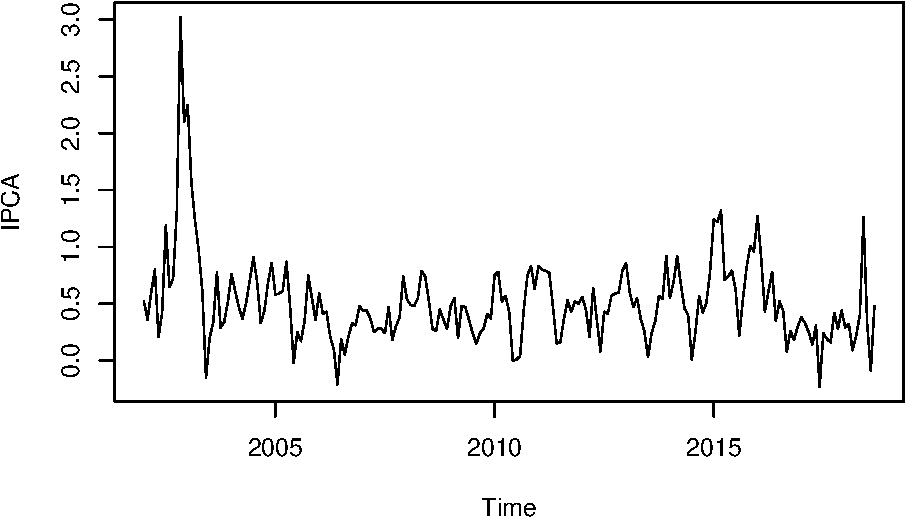
\includegraphics{Bookdown_files/figure-latex/unnamed-chunk-12-1.pdf}

Veja que colocamos o \texttt{View(busca)} comentado apenas para este
post: ao rodar essa linha, uma aba no RStudio abrirá e mostrará todas as
séries que se encaixam neste critério.

Veja que este não é o único pacote disponível para baixar dados! Existem
muitos outros, e a melhor maneira é fuçar o CRAN. (Mas em breve devo
adicionar mais um aqui, o \textbf{Quandl})

\section{Trabalhando com os dados}\label{trabalhando-com-os-dados}

Uma vez carregado os dados, pode ser necessário manipular os dados de
diversas maneiras. Esta seção tratará de algumas das maneiras mais
comuns.

\subsection{Selecionando
linhas/colunas/elementos}\label{selecionando-linhascolunaselementos}

Selecionar uma linha ou uma coluna específica de uma base de dados é
essencial. Se quisermos rodar uma regressão e cada coluna da tabela é
uma variável, então temos que ser capazes de informar ao R quais colunas
serão usadas como variável explicada e quais como variável explicativa.
O R usa a notação de matrizes com colchetes, então para selecionar a 4ª
linha da base de dados chamada dados, basta fazer
\texttt{dados{[}4,{]}}. Veja que colocamos a vírgula e depois deixamos
em branco, informando ao R que queremos todas as colunas. Para obter
todas as linhas da quarta coluna, fazemos \texttt{dados{[},4{]}}.

E se quisermos apenas algumas linhas ou algumas colunas? Podemos passar
um vetor dizendo quais são essas linhas e/ou colunas. Por exemplo, se
quisermos as linhas 1 \textbf{a} 4, podemos passar um
\texttt{dados{[}1:4,{]}}. E se quisermos as linhas 1 \textbf{e} 4,
podemos fazer: \texttt{dados{[}c(1,4),{]}}

Outra maneira, bastante útil, de selecionar variáveis é pelo nome delas.
Suponha que os dados vem com nomes id, renda, escolaridade. Para
selecionar a variável renda, basta fazer \texttt{dados\$renda}. Veja que
isso exige saber como (e se) o R importou os nomes. Para isso, a função
\texttt{names} permite saber quais os nomes das variáveis. Logo
\texttt{names(dados)} vai retornar os nomes das variáveis. Em geral, os
espaços são substituídos por pontos, logo uma variável anos de estudo se
tornará \texttt{anos.de.estudo}. Veja que também podemos acessar as
variáveis em um data.frame usando
\texttt{nome\ do\ data.frame\$nome\ da\ variável}. Assim, se temos um
data.frame com nome dados e queremos acessar a variável renda, bastaria
fazer \texttt{dados\$renda}.

Veja que podemos querer selecionar apenas um elemento. No caso de vetor,
é a única coisa que faz sentido: o vetor só tem uma dimensão (uma linha
ou uma coluna), então só podemos pegar um elemento dele. Suponha que
temos o vetor \(\mathbf{v}\) e queremos o décimo elemento: basta fazer
\texttt{v{[}10{]}}. Veja que não usamos vírgulas, que são usadas apenas
para separar as dimensões. Se quisermos um elemento de uma matriz, basta
passar a linha e a coluna dele, respectivamente. Por exemplo, o elemento
da segunda linha e quinta coluna do dataframe dados é obtido usando
\texttt{dados{[}2,5{]}}.

Mas o R permite você selecionar o elemento de uma matriz como se fosse
um vetor! Suponha uma matriz - chamaremos ela de \(\mathbf{M}\) - com 5
linha e 5 colunas. O último elemento da matriz pode ser obtido com
\texttt{M{[}5,5{]}} ou, equivalentemente, \texttt{M{[}25{]}}. Veja que o
25 não é a toa, no total a matriz tem 25 elementos: logo, o último tem
que ser o membro 25.

\subsection{Criando dummies}

As vezes, queremos transformar uma variável contínua em uma
\emph{dummy}. Pode ser o caso que queremos isolar apenas aqueles que
recebem menos de um salário mínimo, e queremos que quem tiver menos de
um salário mínimo tenha valor 1 e, caso contrário, 0. Suponha que o
salário mínimo seja 678, e que a variável de salários se chame w. Então,
bastaria fazer:

\begin{verbatim}
sal.min <- w < 678
\end{verbatim}

Observe que o R vai gerar um vetor de Verdadeiros e Falso. É possível
converter para numérico, mas não há nenhuma necessidade, uma vez que o R
é capaz de interpretar o verdadeiro ou falso como uma \emph{dummy} na
regressão.

O que estamos fazendo é apenas uma operação de compara cada número do
vetor ao número 678. Testamos se ele é menor (\textless{}), mas
poderíamos ver que números são maiores (\textgreater{}), iguais
(==)\footnote{Dois iguais seguidos}, menor ou igual (\textless{}=) ou
maior ou igual (\textgreater{}=). Estes operadores não são apenas úteis
para criar \emph{dummies}, mas também pode servir para escrever funções,
que será tratado mais a frente.

Pode ocorrer de a variável vir como um vetor de palavras ou siglas.
Suponha que estamos trabalhando com um painel que tem variação temporal
e por estado, e o vetor de estados vem com as siglas dos estados
(RJ,SP,ES,MG,DF\ldots{}). Se quisermos usar efeitos fixos de uma maneira
extremamente ingênua, poderíamos criar dummies para cada estado e
estimar o efeito fixo de cada estado. Esta não é uma maneira inteligente
de fazer, já que existem pacotes para fazer estimação usando efeitos
fixos com bem menos trabalho, que serão tratados no próximo capítulo.
Mas, no momento, vamos ignorar esta opção e tentar criar uma dummy para
cada estado.

Uma possível solução era criar um vetor para cada estado (Ou talvez uma
matriz com n linha e o número de colunas sendo igual o número de
estados), ler cada posição do vetor das siglas usando um loop e colocar
um 1 na coluna correspondente, criando um vetor índice para o R buscar
qual coluna é relacionada com cada estado\ldots{} Se a explicação
anterior bagunçou o seu cérebro, não se preocupe: ela é complicada, e o
R não exige nada tão complicado\footnote{Em geral. O autor já encontrou
  situações em que esse tipo de solução era estritamente necessária.}

Uma solução muito mais simples é usar o comando factors, que gera
automaticamente dummies para cada categoria. Assim, RJ vira uma dummy,
SP outra etc. Isso é automático, e podemos jogar direto numa regressão.
Assim, suponha que temos uma base de dados chama dados e a coluna 2 é a
coluna com os estados. Nesse caso:
\texttt{estados\ \textless{}-\ factor(dados{[},2{]})}. Poderíamos usar
estados diretamente na regressão, que será tratada no capítulo seguinte.

\chapter{Regressão Básica}\label{regressao-basica}

O coração de econometria é o modelo de regressão linear, estimado por
Mínimos Quadrados Ordinários. Mas muitos outros métodos são úteis, como
modelos logit, probit, variáveis instrumentais e modelos para painel.
Este capítulo trata - finalmente! - de modelos de regressão no R.

\section{Mínimos quadrados
ordinários}\label{minimos-quadrados-ordinarios}

Suponha que carregamos uma base de dados (chamada dados), e que esta
base tem as variáveis \(y, x.1,x.2,x.13\) e que nosso objetivo é estimar
um modelo da forma:
\(y = \beta_0 + \beta_1 x_1 + \beta_2 x_2 + \beta_3 x_3 + \epsilon\). O
comando que faz estimativa por mínimos quadrados é o \texttt{lm} e para
estimarmos a regressão proposta basta fazer:

\begin{verbatim}
reg <- lm(y ~ x.1 + x.2 + x.3 + x.4, data = dados)
\end{verbatim}

Usamos o \textasciitilde{} para separar a variável explicada (à esquerda
do til) das explicativas (à direita do til), e para separar as
explicativas usamos o +. A opção \emph{data} diz ao R onde buscar as
variáveis.

Agora, o objeto reg\footnote{Se você leu a discussão anterior de tipos
  de objetos, vale observar que reg é uma lista} tem o modelo estimado.
Para obter uma tabela usual de regressão, com valor do coeficiente, erro
padrão, estatística t e p-valor, \(R^2\) ajustado, e o teste F para os
coeficientes basta usar \texttt{summary(reg)}. No contexto de regressão
linear, podemos querer fazer uma série de coisas, que são explicadas a
seguir.

\textbf{Atenção: Séries Temporais e o lm} Objetos de série temporal são
armazenados pelo R de uma maneira especial - uma vez que você transforma
ele em um objeto de série temporal. Entretanto, você \emph{não} deve
passar um objeto de série temporal para o \texttt{lm()}, já que o
\texttt{lm} vai ignorar o formato de série temporal. Assim, estimar um
modelo AR(1) usando \texttt{lm(y\ \textasciitilde{}\ lag(y))} vai gerar
uma regressão com coeficiente 1 para lag(y) e \(R^2 = 1\). De fato, a
regressão feita foi y em y - o que não é uma regressão muito
emocionante.

\subsection{Testes de hipótese}\label{testes-de-hipotese}

Suponha que queremos testar a significância conjunta de x.2 e x.3.
Precisamos fazer um teste F. Uma maneira é estimar um novo modelo, que
chamaremos de reg.2, só com o x.1:
\texttt{reg.2\ \textless{}-\ lm(y\ \textasciitilde{}\ x.1)}

Agora, para testar a significância conjunta de x.2 e x.3 basta fazer
\texttt{anova(reg,reg.2)} e o R reportará os valores do teste (incluindo
o p valor)

Testes mais gerais também estão disponíveis, pelo pacote car\footnote{Nada
  haver com carro: é uma sigla para Companion to Applied Reggresion}. O
comando é \texttt{linearHypotesis} com o primeiro argumento sendo o
objeto com o modelo. O segundo comando é a hipótese que estamos
testando, entre aspas, e entramos ele de maneira extremamente intuitiva:
suponha que no exemplo acima queremos testar se o coeficiente de x.2 é
igual ao coeficiente de x.4. Nesse caso, o comando se resumiria a
\texttt{linearHypotesis(reg,"x.2\ =\ x.4")}. Várias opções podem ser
usadas, como usar estimadores de erro padrão robustos a
heterocedasticidade. Recomendamos que o leitor olhe o help do comando no
R.

\subsection{Erros padrões robustos}\label{erros-padroes-robustos}

Na presença de heterocedasticidade ou autocorrelação, os erros padrões
usuais não são confiáveis. Infelizmente, o comando \texttt{summary} não
exibe erros robustos por default e nem permite alterar os erros padrões
exibidos. Felizmente, o pacote lmtest traz uma opção para o sumário
padrão do R. A primeira coisa a fazer é carregar o pacote sandwich
(\texttt{library(sandwich)}). O comando é coeftest e a sintaxe é
curiosa. No caso do nosso exemplo, se quisermos obter erros robustos a
heterocedasticidade:

\begin{verbatim}
coeftest(reg, vcov. = vcovHC(reg))
\end{verbatim}

Uma explicação: O comando coeftest chama o comando vcovHC do pacote
sandwich. Por sua vez, o comando vcovHC precisa saber qual o modelo que
vai ter erros robustos. Por isso uma função que recebe uma função. Veja
que se quisermos erros robustos a heterocedasticidade e autocorrelação,
o comando vira vcovHAC.

\subsection{Logs}\label{logs}

Muitas vezes queremos fazer as regressões não com as variáveis em nível,
mas com as variáveis em log. Nesse caso, suponha que queremos a variável
dependente - y - em log. Para isso, basta fazer
\texttt{log.y\ \textless{}-\ log(y)} e a variável log.y vai ser a versão
em log da variável y. Você pode reescrever a regressão como
\texttt{lm(log.y\ \textasciitilde{}\ x.1\ +\ x.2\ +\ x.3)}.

Agora, pode ocorrer de em alguns casos o vetor y ter algum elemento
zero. Mas \(\log(0) = -\infty\). O R tem um elemento Inf (e - Inf) para
esses casos, mas o comando lm vai acusar um erro ao receber um vetor com
algum elemento Inf. A solução é trocar esse valor para alguma coisa,
como um NA, que o R vai ignorar\footnote{Nem sempre o R vai ignorar um
  NA. Isso depende do pacote e das configurações do R}. Para fazer isso,
suponha que o vetor com os Inf seja o log.y do paragrafo anterior.
Precisamos explicar para o R quais casos nós queremos substituir, e isso
é incrivelmente fácil: assim como podemos usar \texttt{log.y{[}1{]}}
para escolher o primeiro elemento do vetor \texttt{log.y}, podemos
colocar entre colchetes uma condição, por exemplo os elementos do vetor
log.y que são iguais a infinito. Já tratamos disso:
\texttt{log.y\ ==\ -Inf} faz esse trabalho. Assim, se quisermos
substituir os elementos de log.y que são iguais a -Inf por NA, basta
usar o seguinte trecho de código:

\begin{verbatim}
 log.y[log.y == -Inf] <- NA
\end{verbatim}

\section{Probits e Logits}\label{probits-e-logits}

Probits e logits também são úteis quando nossa variável dependente é uma
dummy. Sempre podemos usar um modelo de probabilidade linear, e nesse
caso o comando a ser utilizado é o \texttt{lm}. Mas em casos que
queremos usar um probit ou logit, precisamos recorrer ao \texttt{glm},
que tem sintaxe muito parecida com o \texttt{lm}. Mas além de
especificar as variáveis dependentes e independentes, também precisamos
especificar o tipo de regressão, basicamente a distribuição da variável
dependente. No caso de probits e logits, a variável dependente tem
distribuição binomial. Depois, temos que especificar se a função de
probabilidade da variável dependente é probit ou logit. Os comandos para
estimar probits e logits são ilustrados abaixo:

\begin{verbatim}
mod.1 <- glm(y ~x.1 + x.2 + x.3, family = binomial(link = 'probit'))
mod.2 <- glm(y ~x.1 + x.2 + x.3, family = binomial(link = 'logit'))
\end{verbatim}

E como de praxe, podemos usar o comando \texttt{summary} para obter os
coeficientes, desvios padrões e estatísticas t.

\section{Variável instrumental}\label{variavel-instrumental}

Métodos de variável instrumental são muito úteis e populares,
especialmente em casos de endogenidade. Existem várias implementações,
mas para o mínimos quadrados de dois estágios usual, o pacote \emph{AER}
oferece um comando \texttt{ivreg}. A sintaxe é similar ao \texttt{lm},
mas com uma alteração na formula para inserir os instrumentos, que são
separados dos regressores por \textbar{}.

Por exemplo, suponha que temos a variável dependente y, as variáveis
endogenas x.1 e x.2, a variável exogena x.3, e os instrumentos z.1 e
z.2. Nesse caso, o ivreg seria usado:

\begin{verbatim}
modelo <- ivreg(y ~x.1 + x.2 + x.3|z.1+z.2+x.3)
\end{verbatim}

E podemos usar o \texttt{summary} para ver o valor dos coeficientes,
erros padrão e estatísticas t. Observe que o pacote não mostra o valor
do teste F para o primeiro estágio nem de teste de sobre identificação.

\section{Dados em painel}\label{dados-em-painel}

Em muitas aplicações usamos dados em painel - i.e., com dimensão
temporal e cross section. Em geral, esse tipo de aplicação acaba
envolvendo o uso de efeitos fixos. Existem duas maneiras de fazer:
usando o pacote \emph{plm} ou ``na mão'', usando o lm. Não há nenhuma
vantagem de usar o lm ``na mão'', em geral, exceto em casos que temos
mais de duas dimensões ou por algum motivo o \emph{plm} não funciona.
Exploraremos primeiro o uso do plm, que deve satisfazer a maioria dos
usuários. A solução na mão vem depois e pode ser ignorada sem perda de
continuidade.

Supondo que o pacote já foi instalado e carregado, precisamos (i)
explicar para o pacote quais colunas são as colunas com efeitos fixos de
tempo e unidade e (ii) rodar a regressão propriamente dita. Suponha,
como de praxe, que temos um dataframe carregado no R com nome ``dados''.
Suponha que as colunas com as datas e um índice para unidades se chamam
datas e unidades, respectivamente. Veja que essas colunas podem estar em
formato de carácter, e que isso não deve nos preocupar no momento:
poderia ser o caso de a unidade ser estados do país e o código da
unidade ser o código do estado (DF,RJ,SP,\ldots{}). O pacote \emph{plm}
disponibiliza o comando \emph{plm.data}, que converte um data frame de
forma que quando rodarmos a regressão, o R saiba quem são os efeitos
fixos. Assim, vamos criar um dataframe chamado \textbf{dd}:

\begin{verbatim}
dd <- plm.data(dados,c('unidades','datas'))
\end{verbatim}

O primeiro argumento da função é o data.frame a ser convertido, que
contém as colunas para as quais criaremos efeitos fixos. O segundo
argumento da função são as colunas com os efeitos fixos. Veja que a
ordem é unidade e depois a variável temporal. Agora, a estimação do
modelo pode ser feita usando o comando plm, que tem sintaxe muito
similar ao lm: passamos uma formula com a variável dependente e as
independentes, informamos a base de dados - que nesse caso é o objeto
\textbf{dd}, não o objeto dados. Mas temos algumas novas opções: o
método de estimação (em geral estamos interessados em within, o padrão),
mas mais relevante é que efeitos fixos queremos colocar: só para
indivíduo, só para tempo ou ambos. Abaixo, mostramos a sintaxe para cada
um dos casos, respectivamente:

\begin{verbatim}
mod.1 <- plm(y ~x.1 + x.2,data = dd, effect = 'individual')
mod.2 <- plm(y ~x.1 + x.2,data = dd, effect = 'time')
mod.3 <- plm(y ~x.1 + x.2,data = dd, effect = 'twoways')
\end{verbatim}

Como de praxe, podemos usar o comando \texttt{summary} para obter um
sumário da regressão.

\subsection{Painel usando lm*}\label{painel-usando-lm}

Suponha que não conseguimos usar o \emph{plm} por alguma razão. Por
exemplo, podemos querer três efeitos fixos: se tivermos microdados de
escola, podemos querer ter efeito fixo de aluno, escola e tempo. Podemos
implementar isso no braço usando o \texttt{lm}. Lembre-se que, no fundo,
efeitos fixos são mera \emph{dummies}, então se fizermos um modelo
linear com dummies, devemos obter resultados parecidos.

Para ficarmos em terreno conhecido, suponha que só temos dois efeitos
fixos que nos interessam: unidade e tempo. Cada um desses vem codificado
em duas colunas: uma com a data e outra com algum código para a unidade.
Lembrem-se da discussão no capítulo anterior que o \texttt{lm} é capaz
de usar isso e entender como dummies, sem a necessidade de criar várias
variáveis com 0 e 1. Logo, se queremos explicar y usando x como variável
explicativa e efeitos fixos de unidade e tempo, a seguinte regressão
deve bastar:

\begin{verbatim}
modelo <- lm(y ~x +tempo + unidade, data = dados)
\end{verbatim}

E y,x,tempo e unidade estão no dataframe chamado dados, como de praxe.
Algumas diferenças devem ser notadas para o comando plm:

\begin{enumerate}
\def\labelenumi{(\arabic{enumi})}
\tightlist
\item
  O sumário vai ser mais confuso no caso do \texttt{lm}: o \texttt{plm}
  esconde os efeitos fixos, o que não ocorre no caso do \texttt{lm}
\end{enumerate}

Mas mais importante:

\begin{enumerate}
\def\labelenumi{(\arabic{enumi})}
\setcounter{enumi}{1}
\tightlist
\item
  Devido a maneira como o \texttt{plm} estima o modelo (por
  \emph{within}, em geral), o \texttt{plm} usa menos graus de liberdade
  e pode fazer estimações mais precisas. Isso deve impactar mais nos
  desvios padrões que no valor dos coeficientes, especialmente quando o
  número de variáveis for muito grande.
\end{enumerate}

Hands on!

É uma boa hora de checar se os resultados do plm e do lm são de fato
similares. O pacote \emph{AER} traz a base de dados do exemplo de dados
em painel sobre cigarros tirado do livro do Stock e Watson. Para
carregar, basta digitar \texttt{data("CigarettesSW")}. Os efeitos fixos
são para estado e ano, e vem em colunas com nomes state e year,
respectivamente. As variável packs nos traz o número de pacotes
consumido naquele ano e estado, e income a renda do estado naquele ano.
Uma regressão packs em income com efeitos fixos para estado e ano pode
ser feita usando os dois métodos da seção anterior: o \texttt{plm} e o
\texttt{lm}. Ambos devem dar, aproximadamente, o mesmo valor para o
coeficiente do efeito da renda sobre pacotes \((-9.070e-08)\).

\chapter{Séries Temporais}\label{series-temporais}

Métodos de séries temporais são suficientemente extensos e únicos para
terem seu próprio capítulo. Este capítulo trata dos principais métodos
de séries temporais de interesse dos economistas: ARIMAs, VARs, testes
de raiz unitária e cointegração. Séries temporais são únicas o
suficiente a ponto de terem um classe própria - sem nenhuma surpresa,
ela se chama \emph{time series}.

\section{O básico}\label{o-basico}

Suponha que você, usando os métodos do capítulo 2, inseriu uma série
temporal no R. O R não sabe, \emph{a priori}, que os dados são uma série
temporal. Você precisa contar isso a ele, e o comando que faz isso é o
\texttt{ts()}. O \texttt{ts} recebe a série, a data de ínicio e a
frequência. A frequência é como você dividiu o ano: 4 se o dado for
trimestral, 12 se for mensal\ldots{}

Por exemplo, podemos gerar uma série de variáveis aleatórias da normal
(um ruído branco) e transformar em série temporal mensal começando em
janeiro de 2000:

\begin{Shaded}
\begin{Highlighting}[]
\NormalTok{serie <-}\StringTok{ }\KeywordTok{rnorm}\NormalTok{(}\DecValTok{1000}\NormalTok{)}
\NormalTok{serie <-}\StringTok{ }\KeywordTok{ts}\NormalTok{(serie,}\DataTypeTok{start =}\KeywordTok{c}\NormalTok{(}\DecValTok{2000}\NormalTok{,}\DecValTok{01}\NormalTok{), }\DataTypeTok{freq =} \DecValTok{12}\NormalTok{)}
\end{Highlighting}
\end{Shaded}

Veja que o comando ts() é excessivamente engessado: os dados tem que ter
uma frequência fixa, expressa como uma fração do ano. O pacote
\textbf{zoo} extende bastante as capacidades do R em lidar com séries
temporais, inclusive com séries irregulares.

\textbf{Atenção: Séries Temporais e o lm} Você \emph{não} deve passar um
objeto de série temporal para o \texttt{lm()}, já que o \texttt{lm} vai
ignorar o formato de série temporal. Assim, estimar um modelo AR(1)
usando \texttt{lm(y\ \textasciitilde{}\ lag(y))} vai gerar uma regressão
com coeficiente 1 para lag(y) e \(R^2 = 1\). De fato, a regressão feita
foi y em y - o que não é uma regressão muito emocionante.

\section{ARIMAs}\label{arimas}

Com uma série devidamente construída para ser um objeto ts - como nós
fizemos acima- podemos tentar estimar algum modelo. O modelo base de
séries temporais é o ARIMA. O R base já vem com muitas funções para
lidar com isso, mas o pacote \textbf{forecast} extende bastante as
capacidades do R em lidar com esse tipo de série. O primeiro passo para
estimar um modelo Arima é obter a função de autocorrelação (FAC) e a
função de autocorrelação parcial (FACP): elas são \texttt{Acf} e
\texttt{Pacf}. Veja que existem versões na base do R que se chamam
\texttt{acf} e \texttt{pacf} (notem que lá é com maiúscula e aqui com
minúscula). A diferença \emph{fundamental} entre os dois é que a
\texttt{Acf} e a \texttt{acf} (e também a \texttt{Pacf} e a
\texttt{pacf}) é que a primeira exclui a autocorrelação no momento 0 -
que é trivialmente 1.

Uma vez conhecendo o formato da FAC e da FACP, podemos estimar o ARIMA.
O comando para estimar um modelo ARIMA é \texttt{Arima} - e novamente,
existe um \texttt{arima} com minúscula que é da base do R. O
\texttt{Arima} basicamente recebe duas coisas, a série e a ordem do
modelo(isso é, se o modelo é um ARMA(1,1), AR(1), MA(1) etc). Vamos
gerar um exemplo de um AR(1) com dados simulados e obter a FAC e FACP e
estimar o modelo Arma sugerido:

\begin{Shaded}
\begin{Highlighting}[]
\KeywordTok{library}\NormalTok{(forecast)}

\NormalTok{u <-}\StringTok{ }\KeywordTok{rnorm}\NormalTok{(}\DecValTok{500}\NormalTok{)}
\NormalTok{y <-}\StringTok{ }\KeywordTok{rep}\NormalTok{(}\DecValTok{0}\NormalTok{,}\DecValTok{500}\NormalTok{) }\CommentTok{#nossa futura série}

\NormalTok{y[}\DecValTok{1}\NormalTok{] <-}\StringTok{ }\NormalTok{u[}\DecValTok{1}\NormalTok{]}

\ControlFlowTok{for}\NormalTok{(i }\ControlFlowTok{in} \DecValTok{2}\OperatorTok{:}\DecValTok{500}\NormalTok{)\{}
\NormalTok{  y[i] <-}\StringTok{ }\FloatTok{0.6}\OperatorTok{*}\NormalTok{y[i}\OperatorTok{-}\DecValTok{1}\NormalTok{] }\OperatorTok{+}\StringTok{ }\NormalTok{u[i] }\CommentTok{#um AR(1) com coeficiente 0.6}
\NormalTok{\}}

\KeywordTok{Acf}\NormalTok{(y)}
\end{Highlighting}
\end{Shaded}

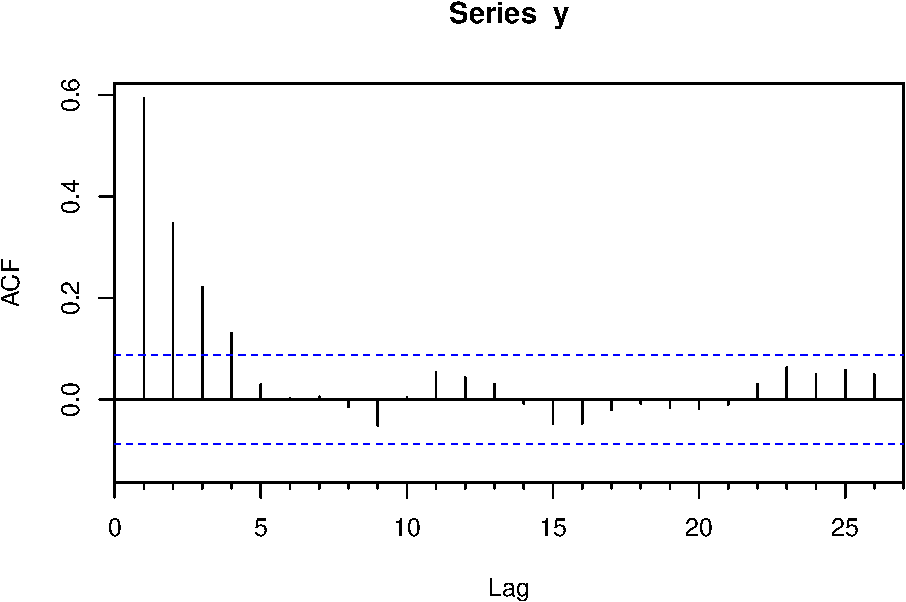
\includegraphics{Bookdown_files/figure-latex/unnamed-chunk-14-1.pdf}

\begin{Shaded}
\begin{Highlighting}[]
\KeywordTok{Pacf}\NormalTok{(y)}
\end{Highlighting}
\end{Shaded}

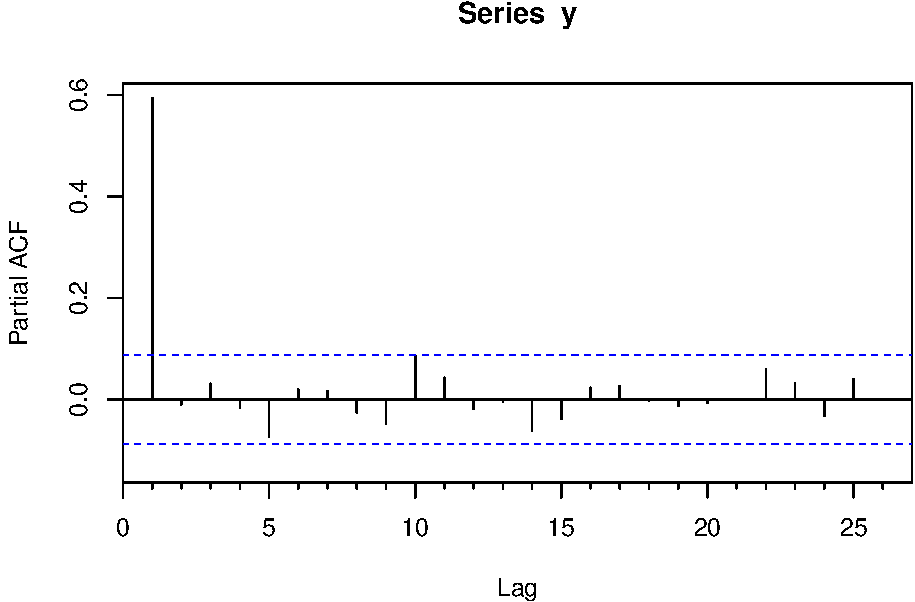
\includegraphics{Bookdown_files/figure-latex/unnamed-chunk-14-2.pdf}

\begin{Shaded}
\begin{Highlighting}[]
\NormalTok{modelo <-}\StringTok{ }\KeywordTok{Arima}\NormalTok{(serie,}\DataTypeTok{order=}\KeywordTok{c}\NormalTok{(}\DecValTok{1}\NormalTok{,}\DecValTok{0}\NormalTok{,}\DecValTok{0}\NormalTok{))}
\KeywordTok{summary}\NormalTok{(modelo)}
\end{Highlighting}
\end{Shaded}

\begin{verbatim}
## Series: serie 
## ARIMA(1,0,0) with non-zero mean 
## 
## Coefficients:
##          ar1   mean
##       0.0083  0.000
## s.e.  0.0317  0.031
## 
## sigma^2 estimated as 0.9467:  log likelihood=-1390.57
## AIC=2787.15   AICc=2787.17   BIC=2801.87
## 
## Training set error measures:
##                         ME      RMSE       MAE      MPE     MAPE      MASE
## Training set -1.697063e-05 0.9720336 0.7874101 99.24187 100.6228 0.6946617
##                      ACF1
## Training set 9.048762e-06
\end{verbatim}

Veja que o objeto \texttt{modelo} trás os coeficientes estimados, o erro
padrão e alguns diagnósticos úteis como critérios de informação.

Em algumas situações pode ser muito difícil inferir o modelo certo a
partir da FAC e da FACP. O comando \texttt{auto.arima}, do pacote
\textbf{forecast}, seleciona um modelo a partir de algum critério de
informação. Vamos ilustrar o ponto gerando uma série \texttt{x} que é um
ARMA(1,2):

\begin{Shaded}
\begin{Highlighting}[]
\NormalTok{e <-}\StringTok{ }\KeywordTok{rnorm}\NormalTok{(}\DecValTok{1000}\NormalTok{)}

\NormalTok{x <-}\StringTok{ }\KeywordTok{rep}\NormalTok{(}\DecValTok{0}\NormalTok{,}\DecValTok{1000}\NormalTok{)}

\ControlFlowTok{for}\NormalTok{(j }\ControlFlowTok{in} \DecValTok{1}\OperatorTok{:}\DecValTok{998}\NormalTok{)\{}
\NormalTok{  x[j}\OperatorTok{+}\DecValTok{2}\NormalTok{] <-}\StringTok{ }\FloatTok{0.5}\OperatorTok{*}\NormalTok{x[j}\OperatorTok{+}\DecValTok{1}\NormalTok{] }\OperatorTok{+}\StringTok{ }\NormalTok{e[j}\OperatorTok{+}\DecValTok{2}\NormalTok{] }\OperatorTok{-}\StringTok{ }\FloatTok{0.3}\OperatorTok{*}\NormalTok{e[j}\OperatorTok{+}\DecValTok{1}\NormalTok{] }\OperatorTok{+}\StringTok{ }\FloatTok{0.4}\OperatorTok{*}\NormalTok{e[j]}
\NormalTok{\}}

\NormalTok{x <-}\StringTok{ }\NormalTok{x[}\DecValTok{500}\OperatorTok{:}\DecValTok{1000}\NormalTok{]}
\NormalTok{x <-}\StringTok{ }\KeywordTok{ts}\NormalTok{(x, }\DataTypeTok{start =} \KeywordTok{c}\NormalTok{(}\DecValTok{1999}\NormalTok{,}\DecValTok{05}\NormalTok{), }\DataTypeTok{freq =} \DecValTok{12}\NormalTok{)}

\KeywordTok{Acf}\NormalTok{(x)}
\end{Highlighting}
\end{Shaded}

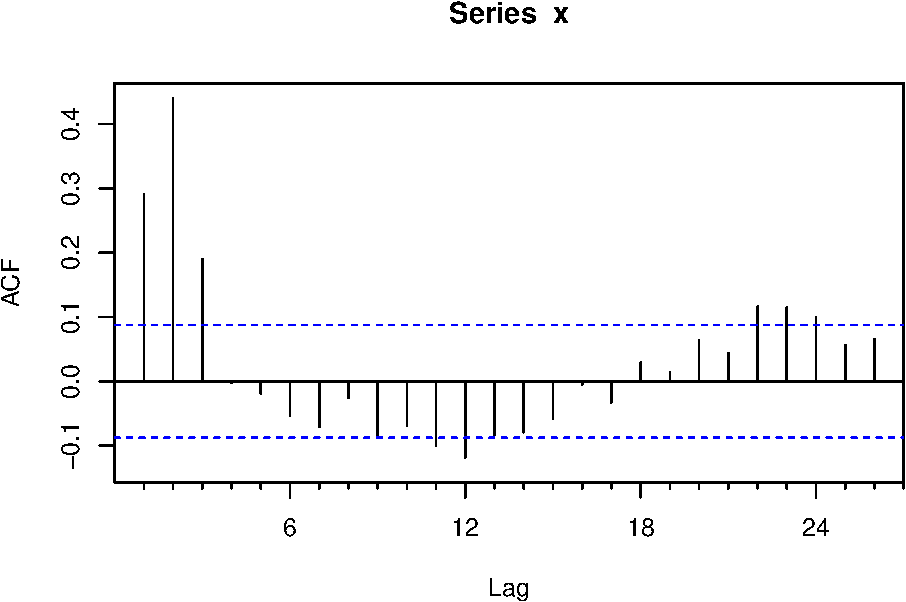
\includegraphics{Bookdown_files/figure-latex/unnamed-chunk-15-1.pdf}

\begin{Shaded}
\begin{Highlighting}[]
\KeywordTok{Pacf}\NormalTok{(x)}
\end{Highlighting}
\end{Shaded}

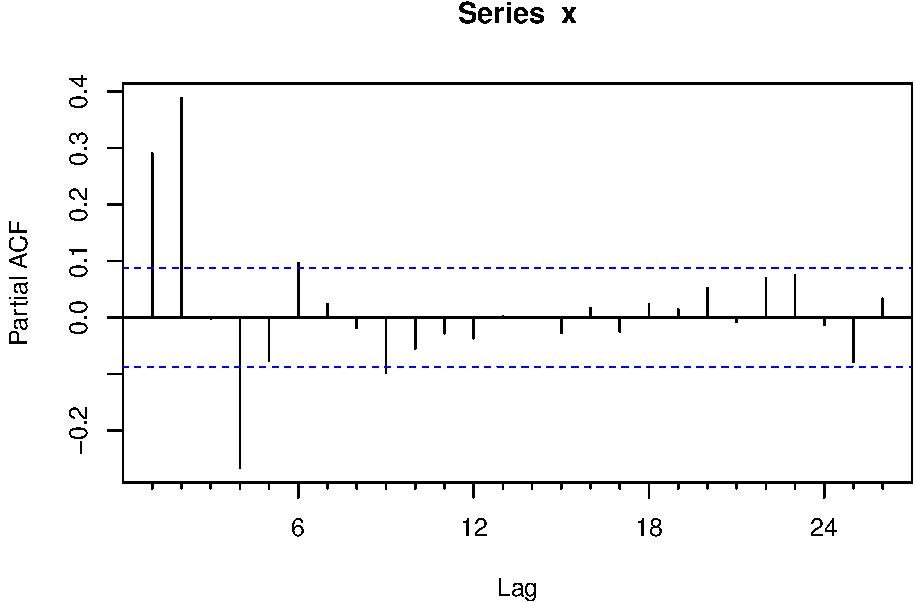
\includegraphics{Bookdown_files/figure-latex/unnamed-chunk-15-2.pdf}

\begin{Shaded}
\begin{Highlighting}[]
\KeywordTok{auto.arima}\NormalTok{(x,}\DataTypeTok{ic =} \StringTok{"bic"}\NormalTok{)}
\end{Highlighting}
\end{Shaded}

\begin{verbatim}
## Series: x 
## ARIMA(1,0,2) with zero mean 
## 
## Coefficients:
##          ar1      ma1     ma2
##       0.4271  -0.2745  0.5143
## s.e.  0.0671   0.0609  0.0393
## 
## sigma^2 estimated as 1.036:  log likelihood=-718.54
## AIC=1445.07   AICc=1445.15   BIC=1461.94
\end{verbatim}

Nesse caso o \texttt{auto.arima} acertou, mas nem sempre isso ocorre.

\section{VARs}\label{vars}

Um VAR, teoricamente, é apenas uma generalização do AR. Ainda assim, do
ponto de vista computacional, eles são distintos, e o VAR tem seu
próprio conjunto de pacotes no R. O mais importante deles é o
\texttt{vars}.

Começamos juntando todas as séries que queremos estimar o VAR em uma
matriz (use o cbind() para isso). O passo seguinte é escolher a ordem do
VAR - geralmente usando algum critério de informação. O comando
\texttt{VARselect} faz isso e apresenta alguns critérios de informação e
a quantidade de lags que minimizam cada um.

O comando que faz a estimativa per se é o \texttt{VAR}. Ele recebe a
matriz com as séries e quantos lags você quer que sejam usados - ou o
critério de informação a ser usado na hora de fazer a estimativa.

Por último, queremos recuperar a resposta dinâmica de cada uma das
variáveis a um choque (não só um choque na própria variável, como o
efeito cruzado de um choque em outra variável).

Vamos gerar um VAR(1) com duas variáveis apenas para ilustrar o uso do
pacote:

\begin{Shaded}
\begin{Highlighting}[]
\KeywordTok{library}\NormalTok{(vars)}

\NormalTok{T <-}\StringTok{ }\DecValTok{500} \CommentTok{#número de períodos}
\NormalTok{N <-}\StringTok{ }\DecValTok{2} \CommentTok{#número de variáveis}

\NormalTok{u <-}\StringTok{ }\KeywordTok{matrix}\NormalTok{(}\KeywordTok{rnorm}\NormalTok{(T}\OperatorTok{*}\NormalTok{N),}\DataTypeTok{nrow =}\NormalTok{ N,}\DataTypeTok{ncol =}\NormalTok{ T)}

\NormalTok{x <-}\StringTok{ }\KeywordTok{matrix}\NormalTok{(}\DecValTok{0}\NormalTok{,}\DataTypeTok{nrow =}\NormalTok{ N, }\DataTypeTok{ncol =}\NormalTok{ T)}

\NormalTok{A <-}\StringTok{ }\KeywordTok{rbind}\NormalTok{(}\KeywordTok{c}\NormalTok{(}\FloatTok{0.3}\NormalTok{,}\OperatorTok{-}\FloatTok{0.2}\NormalTok{),}\KeywordTok{c}\NormalTok{(}\FloatTok{0.6}\NormalTok{,}\FloatTok{0.2}\NormalTok{))}

\ControlFlowTok{for}\NormalTok{(j }\ControlFlowTok{in} \DecValTok{2}\OperatorTok{:}\NormalTok{T)\{}
\NormalTok{  x[,j] <-}\StringTok{ }\NormalTok{A}\OperatorTok\NormalTok{x[,j}\OperatorTok{-}\DecValTok{1}\NormalTok{] }\OperatorTok{+}\StringTok{ }\NormalTok{u[,j]}
\NormalTok{\}}

\NormalTok{x <-}\StringTok{ }\NormalTok{x[,}\DecValTok{400}\OperatorTok{:}\DecValTok{500}\NormalTok{]}
\NormalTok{x <-}\StringTok{ }\KeywordTok{t}\NormalTok{(x)}
\KeywordTok{colnames}\NormalTok{(x) <-}\StringTok{ }\KeywordTok{c}\NormalTok{(}\StringTok{"x"}\NormalTok{,}\StringTok{"y"}\NormalTok{)}

\KeywordTok{VARselect}\NormalTok{(x) }
\end{Highlighting}
\end{Shaded}

\begin{verbatim}
## $selection
## AIC(n)  HQ(n)  SC(n) FPE(n) 
##      2      2      1      2 
## 
## $criteria
##                 1          2          3         4          5          6
## AIC(n) 0.09458332 0.03240114 0.06427672 0.1119467 0.03823184 0.04664907
## HQ(n)  0.16137291 0.14371712 0.22011909 0.3123155 0.28312700 0.33607062
## SC(n)  0.26013449 0.30831977 0.45056280 0.6086003 0.64525282 0.76403750
## FPE(n) 1.09925329 1.03316067 1.06703713 1.1199054 1.04144348 1.05188589
##                7         8          9        10
## AIC(n) 0.1262929 0.1857583 0.09210459 0.1504392
## HQ(n)  0.4602409 0.5642326 0.51510532 0.6179663
## SC(n)  0.9540488 1.1238816 1.14059538 1.3092974
## FPE(n) 1.1415235 1.2148709 1.11023117 1.1821910
\end{verbatim}

\begin{Shaded}
\begin{Highlighting}[]
\NormalTok{modelo <-}\StringTok{ }\KeywordTok{VAR}\NormalTok{(x,}\DataTypeTok{p =} \DecValTok{1}\NormalTok{)}
\KeywordTok{plot}\NormalTok{(}\KeywordTok{irf}\NormalTok{(modelo, }\DataTypeTok{impulse =} \StringTok{"x"}\NormalTok{, }\DataTypeTok{response =} \KeywordTok{c}\NormalTok{(}\StringTok{"x"}\NormalTok{,}\StringTok{"y"}\NormalTok{)))}
\end{Highlighting}
\end{Shaded}

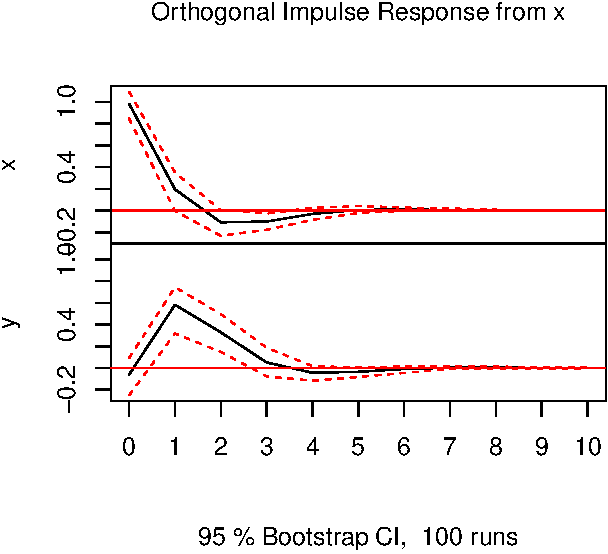
\includegraphics{Bookdown_files/figure-latex/unnamed-chunk-16-1.pdf}

Eu só pedi o plot do choque da primeira variável sobre as duas variáveis
por que isso é uma ilustração. Fazer \texttt{plot(irf(modelo))} em uma
seção do R, ele vai plotar os choques de todas as variáveis sobre todas
as variáveis.

\section{Raiz unitária}\label{raiz-unitaria}

O pacote \textbf{urca} nos trás testes de raiz unitária. O teste
Dickey-Fuller, um dos mais populares, é chamado pelo \texttt{ur.df()}.
Vamos gerar um passeio aleatório para mostrar:

\begin{Shaded}
\begin{Highlighting}[]
\NormalTok{ x <-}\StringTok{ }\KeywordTok{cumsum}\NormalTok{(}\KeywordTok{rnorm}\NormalTok{(}\DecValTok{1000}\NormalTok{))}
\KeywordTok{summary}\NormalTok{(}\KeywordTok{ur.df}\NormalTok{(x))}
\end{Highlighting}
\end{Shaded}

\begin{verbatim}
## 
## ############################################### 
## # Augmented Dickey-Fuller Test Unit Root Test # 
## ############################################### 
## 
## Test regression none 
## 
## 
## Call:
## lm(formula = z.diff ~ z.lag.1 - 1 + z.diff.lag)
## 
## Residuals:
##     Min      1Q  Median      3Q     Max 
## -3.1685 -0.7405 -0.0154  0.6057  3.3920 
## 
## Coefficients:
##              Estimate Std. Error t value Pr(>|t|)
## z.lag.1     0.0002941  0.0024743   0.119    0.905
## z.diff.lag -0.0176797  0.0317600  -0.557    0.578
## 
## Residual standard error: 0.9862 on 996 degrees of freedom
## Multiple R-squared:  0.0003166,  Adjusted R-squared:  -0.001691 
## F-statistic: 0.1577 on 2 and 996 DF,  p-value: 0.8541
## 
## 
## Value of test-statistic is: 0.1189 
## 
## Critical values for test statistics: 
##       1pct  5pct 10pct
## tau1 -2.58 -1.95 -1.62
\end{verbatim}

Veja que o valor crítico para o teste Dick Fuller não é o valor usual da
estatística t, mas sim o valor exibido na parte debaixo da tabela do
sumário do teste. Nesse caso, a qualquer nível de significância, nós não
rejeitamos a hipótese de raiz unitária. Vamos testar para um caso
estacionário:

\begin{Shaded}
\begin{Highlighting}[]
\NormalTok{u <-}\StringTok{ }\KeywordTok{rnorm}\NormalTok{(}\DecValTok{2000}\NormalTok{)}
\NormalTok{y <-}\StringTok{ }\KeywordTok{rep}\NormalTok{(}\DecValTok{0}\NormalTok{,}\DecValTok{2000}\NormalTok{)}

\ControlFlowTok{for}\NormalTok{(i }\ControlFlowTok{in} \DecValTok{2}\OperatorTok{:}\DecValTok{2000}\NormalTok{)\{}
\NormalTok{  y[i] <-}\StringTok{ }\FloatTok{0.5}\OperatorTok{*}\NormalTok{y[i}\OperatorTok{-}\DecValTok{1}\NormalTok{] }\OperatorTok{+}\StringTok{ }\NormalTok{u[i]}
\NormalTok{\}}

\NormalTok{y <-}\StringTok{ }\NormalTok{y[}\DecValTok{1000}\OperatorTok{:}\DecValTok{2000}\NormalTok{]}

\KeywordTok{summary}\NormalTok{(}\KeywordTok{ur.df}\NormalTok{(y))}
\end{Highlighting}
\end{Shaded}

\begin{verbatim}
## 
## ############################################### 
## # Augmented Dickey-Fuller Test Unit Root Test # 
## ############################################### 
## 
## Test regression none 
## 
## 
## Call:
## lm(formula = z.diff ~ z.lag.1 - 1 + z.diff.lag)
## 
## Residuals:
##     Min      1Q  Median      3Q     Max 
## -4.2628 -0.7098  0.0215  0.7612  3.1409 
## 
## Coefficients:
##            Estimate Std. Error t value Pr(>|t|)    
## z.lag.1    -0.48838    0.03093 -15.792   <2e-16 ***
## z.diff.lag  0.02522    0.03170   0.796    0.426    
## ---
## Signif. codes:  0 '***' 0.001 '**' 0.01 '*' 0.05 '.' 0.1 ' ' 1
## 
## Residual standard error: 1.081 on 997 degrees of freedom
## Multiple R-squared:  0.2387, Adjusted R-squared:  0.2372 
## F-statistic: 156.3 on 2 and 997 DF,  p-value: < 2.2e-16
## 
## 
## Value of test-statistic is: -15.7924 
## 
## Critical values for test statistics: 
##       1pct  5pct 10pct
## tau1 -2.58 -1.95 -1.62
\end{verbatim}

\section{Desassonalizando}\label{desassonalizando}

Dados de séries temporais, não raramente, apresentam sazonalidade. Por
exemplo, gasto de energia elétrica tende a ser maior nos meses de
dezembro a fevereiro, devido ao verão. Retirar sazonalidade é importante
em muitas análises.

Um método padrão é colocar \emph{dummies} para as unidades de tempo (uma
para cada mês se o dado for mensal, uma para cada trimestre se for
trimestral etc) e usar o \emph{resíduo} dessa regressão somado a média
da série (já que o resíduo tem média zero, por construção). Criar as
\emph{dummies} ``no braço'' pode ser tedioso, mas felizmente o pacote
\textbf{forecast} trás o comando \texttt{seasonaldummy()} que cria as
\emph{dummies} automaticamente para a série.

\begin{Shaded}
\begin{Highlighting}[]
\NormalTok{energia <-}\StringTok{ }\KeywordTok{BETSget}\NormalTok{(}\DecValTok{1406}\NormalTok{, }\DataTypeTok{from =} \StringTok{"2002-01-01"}\NormalTok{)}
\NormalTok{dum <-}\StringTok{ }\KeywordTok{seasonaldummy}\NormalTok{(energia)}
\NormalTok{mod <-}\StringTok{ }\KeywordTok{Arima}\NormalTok{(energia, }\DataTypeTok{xreg =}\NormalTok{ dum)}
\NormalTok{des <-}\StringTok{ }\KeywordTok{resid}\NormalTok{(mod) }\OperatorTok{+}\StringTok{ }\KeywordTok{mean}\NormalTok{(energia)}
\KeywordTok{plot}\NormalTok{(energia)}
\KeywordTok{lines}\NormalTok{(des, }\DataTypeTok{col =} \DecValTok{2}\NormalTok{)}
\KeywordTok{legend}\NormalTok{(}\StringTok{"topleft"}\NormalTok{, }\DataTypeTok{legend =} \KeywordTok{c}\NormalTok{(}\StringTok{"C/Sazonalidade"}\NormalTok{, }\StringTok{"Sem Sazonalidade"}\NormalTok{), }\DataTypeTok{lty =} \KeywordTok{c}\NormalTok{(}\DecValTok{1}\NormalTok{,}\DecValTok{1}\NormalTok{), }\DataTypeTok{col =} \KeywordTok{c}\NormalTok{(}\DecValTok{1}\NormalTok{,}\DecValTok{2}\NormalTok{))}
\end{Highlighting}
\end{Shaded}

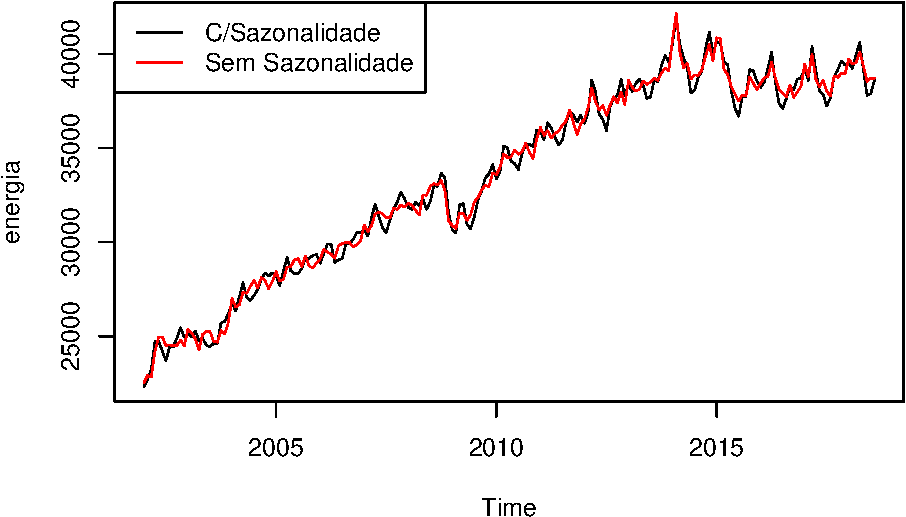
\includegraphics{Bookdown_files/figure-latex/desazonalizando-1.pdf}

Outra maneira comum de dessazonalizar é usando o X13, um programa do
governo americano. O X13 pode ser acessado direto do R usando o pacote
\textbf{seasonal}. O comando que acessa o X13 é o \texttt{seas}. O X13
são, na verdade, \emph{dois} programas: um que é o X13 e o outro que é o
SEATS. Ambos tem a mesma função: dessazonalizar. O X13 vem com todo tipo
de método automático para detectar outliers, fazer transformações nas
séries e uma infinidade de outras coisas. Nesse caso, nós vamos desligar
todas essa opções:

\begin{Shaded}
\begin{Highlighting}[]
\KeywordTok{library}\NormalTok{(seasonal)}
\NormalTok{modelo2 <-}\StringTok{ }\KeywordTok{seas}\NormalTok{(energia, }\DataTypeTok{transform.function =} \StringTok{"none"}\NormalTok{, }\DataTypeTok{regression.aictest =} \OtherTok{NULL}\NormalTok{, }\DataTypeTok{outlier =} \OtherTok{NULL}\NormalTok{)}
\end{Highlighting}
\end{Shaded}

O comando \texttt{final} obtém a série dessazonalizada:

\begin{Shaded}
\begin{Highlighting}[]
\KeywordTok{plot}\NormalTok{(energia)}
\KeywordTok{lines}\NormalTok{(}\KeywordTok{final}\NormalTok{(modelo2), }\DataTypeTok{col =} \DecValTok{2}\NormalTok{)}
\KeywordTok{legend}\NormalTok{(}\StringTok{"topleft"}\NormalTok{, }\DataTypeTok{legend =} \KeywordTok{c}\NormalTok{(}\StringTok{"C/Sazonalidade"}\NormalTok{, }\StringTok{"Sem Sazonalidade"}\NormalTok{), }\DataTypeTok{lty =} \KeywordTok{c}\NormalTok{(}\DecValTok{1}\NormalTok{,}\DecValTok{1}\NormalTok{), }\DataTypeTok{col =} \KeywordTok{c}\NormalTok{(}\DecValTok{1}\NormalTok{,}\DecValTok{2}\NormalTok{))}
\end{Highlighting}
\end{Shaded}

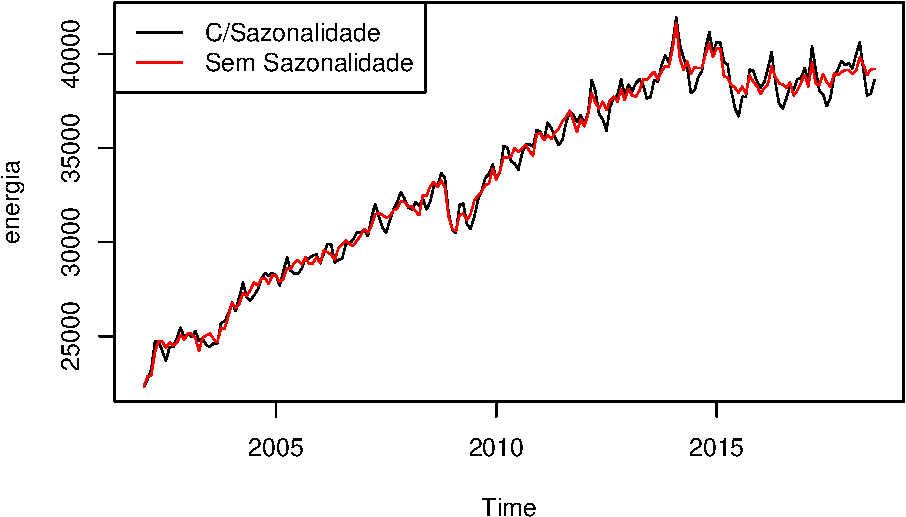
\includegraphics{Bookdown_files/figure-latex/unnamed-chunk-20-1.pdf}

\section{Filtro Hodrick-Prescott}\label{filtro-hodrick-prescott}

O filtro Hodrick-Prescott (HP) é utilizado em séries não estacionárias
quando queremos separar a tendência do componente ciclíco. Ele é
polêmico, mas ainda é amplamente usado. No R, o pacote \textbf{mFilter}
implementa ele e alguns outros. Vamos aplicar na série de energia:

\begin{Shaded}
\begin{Highlighting}[]
\KeywordTok{library}\NormalTok{(mFilter)}
\NormalTok{filtrado <-}\StringTok{ }\KeywordTok{mFilter}\NormalTok{(energia, }\StringTok{"HP"}\NormalTok{)}
\KeywordTok{plot}\NormalTok{(filtrado)}
\end{Highlighting}
\end{Shaded}

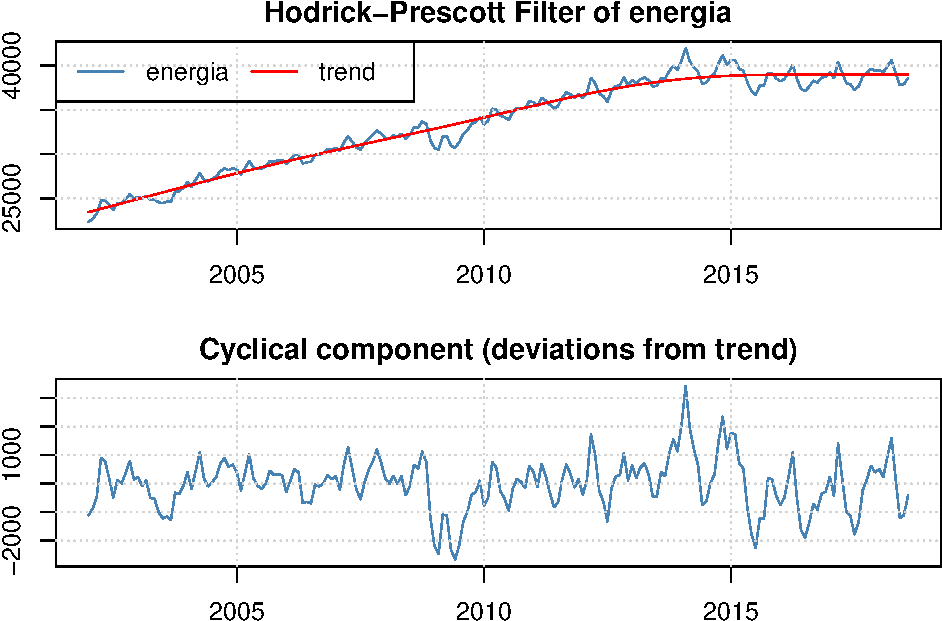
\includegraphics{Bookdown_files/figure-latex/unnamed-chunk-21-1.pdf}

Eu posso acessar a tendência e o componente cíclico usando o
\texttt{filtrado\$trend} e \texttt{filtrado\$cycle}, no exemplo acima -
que seria particularmente útil se eu quisesse utilizar os dados de cíclo
para alguma estimação.

\chapter{Apresentando os resultados}\label{apresentando-os-resultados}

Os milhares de modelos que você rodou são tão úteis quanto a sua
capacidade de apresentar eles. Sem sermos capazes de apresentar os
resultados, nosso trabalho é estéril. Este capítulo apresenta algumas
maneiras de usar o R para apresentar resultados.

\section{Tabelas}\label{tabelas}

Feitas as regressões, precisamos apesentar os resultados. Você sempre
pode copiar e colar o sumário do R, mas convenhamos: ele é feio. Podemos
digitar na mão, mas isto é trabalhoso. A boa notícia é que alguns
pacotes do R ajudam ao criar tabelas. Damos atenção a dois: o
\textbf{stargazer} e o \textbf{xtable}.

A má notícia é que esses dois pacotes não geram tabelas para o Word.
Eles geram tabelas para LaTeX e para html. LaTeX é uma linguagem muito
popular para escrever artigos científicos e livros - este manual foi,
originalmente, escrito em LaTeX; já html é a linguagem padrão para criar
sites na internet, e é a base do Markdown, apresentado na próxima seção.
O que vemos nos documentos como esse e como sites da internet são as
versões compiladas. Tanto html, Markdown e LaTeX não são como o Word,
que o que você vê é como vai ficar no documento final: ambas são, de
certa forma, linguagens de programação para produzir textos. Há um
comando para colocar as palavras em negrito, outro para itálico etc.

Explicar como usar o LaTeX foge do escopo deste manual. Entretanto, o
autor incentiva que o leitor aprenda LaTeX ou Markdown. O Markdown, que
vai ser apresentado com mais detalhes na próxima seção, é um passo
intermediário entre o R e o LaTeX, e pode facilitar imensamente o
aprendizado do LaTeX. Alguns motivos para aprender LaTeX (e Markdown) é
que (1) é mais fácil digitar equações, (2) fácil de integrar com o R,
(3) uma vez que você aprende, é mais fácil que o Word, (4) os documentos
em LaTeX são mais bonitos que os efeitos em Word. As referências no fim
do manual trazem alguns links para os interessados em aprender LaTeX.

O \textbf{xtable} converte tabelas do R para o formato LaTeX. Se você
tem uma matriz de nome \texttt{matriz} e fizer \texttt{xtable(matriz)},
o R vai fornecer o código em LaTeX para fazer uma tabela com os
elementos da \texttt{matriz}. Já o \textbf{stargazer} apresenta o
sumário da regressão em formato LaTeX (ou html) automaticamente. Suponha
que você tenha um modelo chamado \texttt{modelo}. Usar
\texttt{stargazer(modelo)} vai apresentar o sumário do modelo. O comando
é altamente configurável, com uma infinidade de parâmetros; e funciona
com vários pacotes e não só com comandos da base do R, como o
\texttt{lm}.

\section{Markdown}\label{markdown}

O Rstudio já vem com uma opção para trabalhar com arquivos markdown, e
para criar um novo arquivo markdown basta ir no menu, new file, R
Markdown. O R Markdown também depende de comandos para fazer as
alterações no texto - por exemplo, itálico são asteriscos cercando o
texto. Assim, se digitarmos no markdown \texttt{*itálico*}, o resultado
final seria \emph{itálico}. Isso pode parecer esquisito a primeira
vista, mas uma vez criado o hábito, o comportamento é bem mais
previsível que o word.

O Markdown é mais fácil de usar que o LaTeX, mas tem menos opções. O
Rstudio tem várias dicas de como usar o Markdown - basta olhar o help do
Rstudio, ir na opção cheatsheets, e temos duas opções: R Markdown
Cheatsheet e R Markdown Reference Guide. Ambos são úteis. Também no help
temos o Markdown Quick Reference, que tem os principais comandos para o
Markdown, e que abre na mesma janela que o help do R.

Veja que ao criar um novo arquivo, ele dá várias opções: html, pdf,
word. Se você escolher html, pode gerar um pdf ou arquivo word depois,
\emph{mas não o contrário}. Logo, escolha o html. Se você não fez
nenhuma alteração na organização do RStudio, ele deve abrir em cima do
console. Há várias opções na barra abaixo do nome do arquivo e a mais
importante é o Knit: ele vai gerar o documento que você quer ver. Na
primeira vez que você clicar nele, você vai ter que salvar o arquivo: dê
um nome e não esqueça de colocar a extensão .Rmd. Assim, se o arquivo se
chama relatório, você deve salvar como relatorio.Rmd\footnote{Espaços,
  cedilhas e acentos são normalmente uma má ideia em nomes de arquivos.}.
Se tudo der certo, o R vai abrir o novo arquivo, devidamente formatado.
Ele terá o mesmo nome que o arquivo que você salvou. Assim, você terá
dois arquivos: o .Rmd e o .html - assim como, quando geramos um pdf a
partir do word, temos um arquivo .docx e um .pdf. A ideia é a mesma: é
possível editar o .Rmd e gerar o html a partir dele. Veja que é possível
que ele dê algum erro - exatamente como quando rodamos um programa no R.

A parte mais interessante do Markdown é que é possível colocar pedaços
de código do R (e até mesmo de outras linguagens) no meio do texto, e o
Markdown vai ``dar'' esse pedaço de código para o R rodar e reportar o
resultado. Veja o help do Markdown sobre como fazer isso. Apesar de ser
uma possibilidade interessante, ela pode ser problemática: se algum
pedaço do seu código demorar muito para rodar, toda vez que ocê der Knit
o código vai ser rodado. A opção \texttt{cache\ =\ TRUE} no bloco deve
amenizar isso.

\section{Gráficos}\label{graficos}

Outra ferramenta fundamental para apresentar resultados são gráficos. O
R tem um pacote padrão para gráficos e um pacote extra amplamente usado
chamado \textbf{ggplot2}. Neste manual não irei tratar do
\textbf{ggplot2}: o R Studio tem um help excelente que introduz o uso do
\textbf{ggplot2}.

Os gráficos do R são feitos em camadas: a primeira camada é feita com o
comando \texttt{plot}; para adicionar novas coisas na mesma imagem,
existe uma série de outros comandos. Usar o \texttt{plot} de novo vai
gerar uma nova imagem.

Em geral, o \texttt{plot} recebe qual(is) série(s) serão exibidas. Você
pode passar uma única série, que será \emph{plotada} no eixo y, e o eixo
x será apenas o número da observação; ou x e y, e o gráfico vai mostrar
os pontos com coordenadas (x,y). Cada um dos casos, respectivamente:

\begin{Shaded}
\begin{Highlighting}[]
\NormalTok{x <-}\StringTok{ }\KeywordTok{rnorm}\NormalTok{(}\DecValTok{100}\NormalTok{) }\CommentTok{#Gerando alguns números de uma normal}
\NormalTok{y <-}\StringTok{ }\DecValTok{2}\OperatorTok{*}\NormalTok{x}\OperatorTok{+}\KeywordTok{rnorm}\NormalTok{(}\DecValTok{100}\NormalTok{) }\CommentTok{#y é uma função de x com algum erro adicionado}
\KeywordTok{plot}\NormalTok{(y)}
\end{Highlighting}
\end{Shaded}

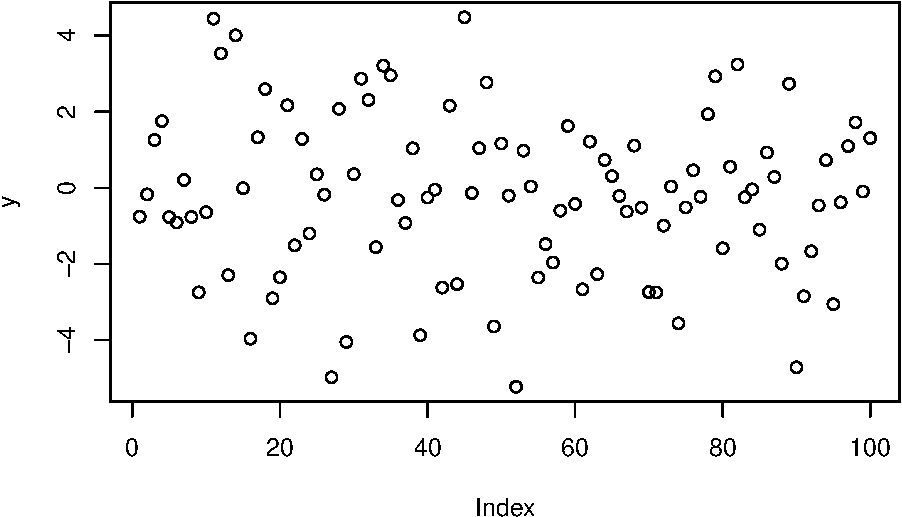
\includegraphics{Bookdown_files/figure-latex/unnamed-chunk-22-1.pdf}

\begin{Shaded}
\begin{Highlighting}[]
\KeywordTok{plot}\NormalTok{(x,y)}
\end{Highlighting}
\end{Shaded}

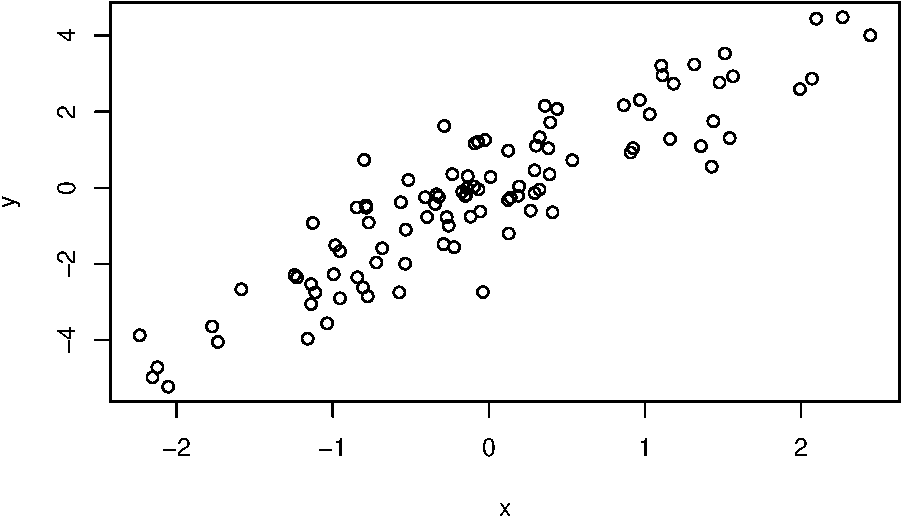
\includegraphics{Bookdown_files/figure-latex/unnamed-chunk-22-2.pdf}

O comando \textbf{plot} tem uma opção especial chamada \textbf{type}.
Aqui você pode escolher como os dados são \emph{plotados}: em pontos, em
linhas ou diversas outras opções descritas no help. O padrão é pontos.
Em geral, se passa a primeira letra de cada tipo. Assim, para fazer o
gráfico de linha da variável y, basta usar
\texttt{plot(y,\ type=\textquotesingle{}\textquotesingle{}l\textquotesingle{}\textquotesingle{})}:

\begin{Shaded}
\begin{Highlighting}[]
\KeywordTok{plot}\NormalTok{(y,}\DataTypeTok{type=}\StringTok{"l"}\NormalTok{)}
\end{Highlighting}
\end{Shaded}

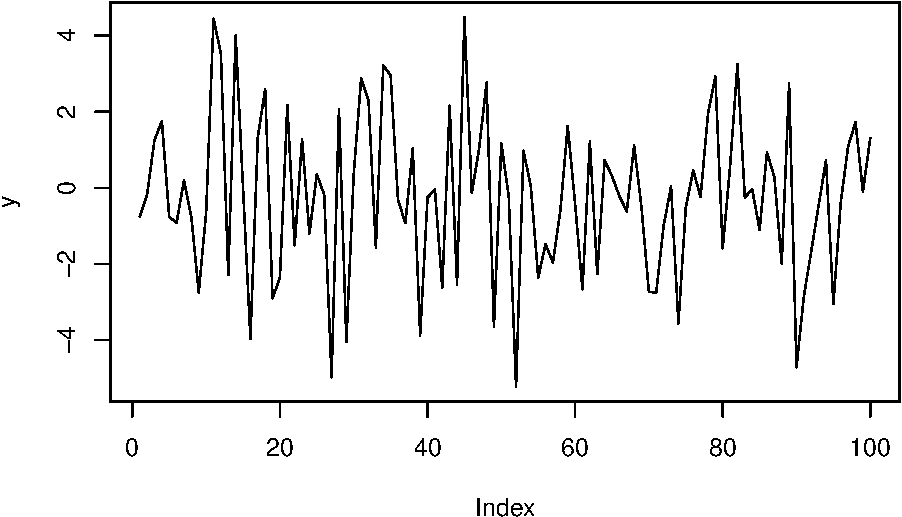
\includegraphics{Bookdown_files/figure-latex/unnamed-chunk-23-1.pdf}

Existem vários comandos para colocar novos objetos sobre o gráfico, mas
vou me limitar a dois: \texttt{points} e \texttt{lines}, que adicionam
respectivamente\ldots{} pontos e linhas. Em geral, \texttt{plot,lines} e
\texttt{points} recebem argumentos parecidos:

\begin{itemize}
\tightlist
\item
  \textbf{col} específica a cor. Em geral, se usa números: 1 é preto, 2
  é vermelho\ldots{}
\item
  \textbf{lty} específica o tipo da linha: logo, é inútil para o comando
  \texttt{points} ou \texttt{plot} sem type=``l''. Também usamos
  números: 1 é a linha sólida, 2 é a linha tracejada\ldots{}
\item
  \textbf{pch} é a contraparte do lty para pontos e permite escolher
  qual o tipo de ponto que será usado no comando \texttt{points} ou no
  \texttt{plot} com opção type = ``p''. Também se usa números para
  especificar como serão os pontos
\end{itemize}

Cada comando gráfico tem suas particularidades e uma visita ao help de
cada um deles é sempre necessária para o autor deste manual.

\chapter{Ifs, Fors, Whiles}\label{ifs-fors-whiles}

Todas as linguagens de programação usam \emph{ifs, fors} e
\emph{whiles}, que sempre fazem a mesma coisa em linhas gerais. Este
capítulo trata deles. Cada seção vai tratar de cada um deles, e todas
serão estruturadas da seguinte maneira: primeiramente, só apresentamos a
sintaxe dos comandos no R. A seguir, temos uma discussão sobre o que
cada estrutura faz. Desta maneira, aqueles que já conhecem essas
estruturas de outras linguagens podem simplesmente ler a sintaxe e pular
toda a discussão subsequente.

Em geral, os exemplos podem não parecer ter utilidade prática, mas
servem para entender as ideias. Aplicações práticas são encontradas nos
capítulos subsequentes.

\section{If}\label{if}

\emph{Ifs} são estruturas condicionais: se essa condição é atendida,
faça isso. Senão, faça aquilo outro. A sintaxe é:

\begin{verbatim}
if(condição){
    ação se a condição for atendida} else {
    ação se a condição não for atendida}
\end{verbatim}

Por exemplo, podemos escrever um código que testa se \(x\) - que deve
ser um número - é igual a 18, e se sim ele nos mostra um ``Sim''. Caso
contrário, ``Não''.

\begin{Shaded}
\begin{Highlighting}[]
\NormalTok{x <-}\StringTok{ }\DecValTok{18}
\ControlFlowTok{if}\NormalTok{(x}\OperatorTok{==}\DecValTok{18}\NormalTok{)\{}
    \KeywordTok{print}\NormalTok{(}\StringTok{"Sim"}\NormalTok{)\} }\ControlFlowTok{else}\NormalTok{ \{}
    \KeywordTok{print}\NormalTok{(}\StringTok{"Não"}\NormalTok{)\}}
\end{Highlighting}
\end{Shaded}

\begin{verbatim}
## [1] "Sim"
\end{verbatim}

\begin{Shaded}
\begin{Highlighting}[]
\NormalTok{x <-}\StringTok{ }\DecValTok{21}
\ControlFlowTok{if}\NormalTok{(x}\OperatorTok{==}\DecValTok{18}\NormalTok{)\{}
    \KeywordTok{print}\NormalTok{(}\StringTok{"Sim"}\NormalTok{)\} }\ControlFlowTok{else}\NormalTok{ \{}
    \KeywordTok{print}\NormalTok{(}\StringTok{"Não"}\NormalTok{)\}}
\end{Highlighting}
\end{Shaded}

\begin{verbatim}
## [1] "Não"
\end{verbatim}

Podemos concatenar vários else e ifs e testar várias condições. Podemos
querer saber se x é menor que 5 ou maior que 7:

\begin{Shaded}
\begin{Highlighting}[]
\NormalTok{x <-}\StringTok{ }\DecValTok{5}
\ControlFlowTok{if}\NormalTok{(x }\OperatorTok{<}\StringTok{ }\DecValTok{5}\NormalTok{)\{}
    \KeywordTok{print}\NormalTok{(}\StringTok{"Menor que 5"}\NormalTok{)\} }\ControlFlowTok{else} \ControlFlowTok{if}\NormalTok{(x }\OperatorTok{>}\StringTok{ }\DecValTok{7}\NormalTok{)\{}
    \KeywordTok{print}\NormalTok{(}\StringTok{"Maior que 7"}\NormalTok{)\} }\ControlFlowTok{else}\NormalTok{ \{}
    \KeywordTok{print}\NormalTok{(}\StringTok{"Nenhum dos dois"}\NormalTok{)\}}
\end{Highlighting}
\end{Shaded}

\begin{verbatim}
## [1] "Nenhum dos dois"
\end{verbatim}

\begin{Shaded}
\begin{Highlighting}[]
\NormalTok{x <-}\StringTok{ }\DecValTok{8}
\ControlFlowTok{if}\NormalTok{(x }\OperatorTok{<}\StringTok{ }\DecValTok{5}\NormalTok{)\{}
    \KeywordTok{print}\NormalTok{(}\StringTok{"Menor que 5"}\NormalTok{)\} }\ControlFlowTok{else} \ControlFlowTok{if}\NormalTok{(x }\OperatorTok{>}\StringTok{ }\DecValTok{7}\NormalTok{)\{}
    \KeywordTok{print}\NormalTok{(}\StringTok{"Maior que 7"}\NormalTok{)\} }\ControlFlowTok{else}\NormalTok{ \{}
    \KeywordTok{print}\NormalTok{(}\StringTok{"Nenhum dos dois"}\NormalTok{)\}}
\end{Highlighting}
\end{Shaded}

\begin{verbatim}
## [1] "Maior que 7"
\end{verbatim}

Essa estrutura pode ser chata e requerer muitas linhas quando queremos
algo simples. Pense no caso que queremos definir a variável h como 1 se
x é maior que 1, e 0 caso contrário. Felizmente, o comando
\texttt{ifelse} resolve isso. A sintaxe dele é simples: a condição, o
valor se a condição for atendida e o valor se a condição não for
atendida. Assim, no exemplo acima:

\begin{Shaded}
\begin{Highlighting}[]
\NormalTok{h <-}\StringTok{ }\KeywordTok{ifelse}\NormalTok{(x }\OperatorTok{>}\StringTok{ }\DecValTok{1}\NormalTok{ ,}\DecValTok{1}\NormalTok{,}\DecValTok{0}\NormalTok{)}
\NormalTok{h}
\end{Highlighting}
\end{Shaded}

\begin{verbatim}
## [1] 1
\end{verbatim}

Entretanto, em muitas situações, usar a estrutura do if ao invés da
função \texttt{ifelse()} é útil.

\section{For e While}\label{for-e-while}

\emph{For} (e \emph{whiles}) são \emph{loops}: eles permitem repetir a
mesma operação várias vezes. Para eles serem interessantes, eles tem que
permitir alguma alteração no input e no output. A sintaxe do for é:

\begin{verbatim}
for(i in 1:n){
ações...
}
\end{verbatim}

Veja que podemos indexar o for por qualquer letra (e não apenas i), e
que podemos usar um vetor para indexar o for, o que vai fazer o for
repetir a operação pelo comprimento daquele vetor - e definir o valor de
i como o valor dos elementos do vetor. Por exemplo:

\begin{Shaded}
\begin{Highlighting}[]
\NormalTok{a <-}\StringTok{ }\KeywordTok{c}\NormalTok{(}\DecValTok{1}\NormalTok{,}\DecValTok{2}\NormalTok{,}\DecValTok{3}\NormalTok{,}\DecValTok{4}\NormalTok{,}\DecValTok{5}\NormalTok{)}
\NormalTok{b <-}\StringTok{ }\DecValTok{0}

\ControlFlowTok{for}\NormalTok{(i }\ControlFlowTok{in}\NormalTok{ a)\{}
\NormalTok{b <-}\StringTok{ }\NormalTok{b }\OperatorTok{+}\StringTok{ }\NormalTok{i}
\KeywordTok{print}\NormalTok{(b)}
\NormalTok{\}}
\end{Highlighting}
\end{Shaded}

\begin{verbatim}
## [1] 1
## [1] 3
## [1] 6
## [1] 10
## [1] 15
\end{verbatim}

Hands on!

Podemos usar o \emph{for} para ilustrar uma ideia bastante importante de
estatística: a lei dos grandes números. Para refrescar a memória: a lei
dos grandes números diz que se a variável aleatória tem média \(\mu\),
\(\bar{X}\) é a média amostral e \(n\) é o tamanho da amostra, então
\(\text{plim}_{n \rightarrow \infty}(\bar{X}) = \mu\). O código para
ilustrar isso é simples:

\begin{itemize}
\tightlist
\item
  Gere um vetor de variáveis aleatórias retirados de alguma distribuição
  (por exemplo, \texttt{rnorm(200)}). Vamos chamar esse vetor de
  \texttt{amostra}.
\item
  Crie um vetor de zeros (você pode fazer isso usando
  \texttt{rep(0,200)}) Chame ele de alguma coisa. No caso, chamarei ele
  de \texttt{media}
\item
  Crie um loop que faz com que cada posição do vetor \texttt{media} seja
  a média dos números em \texttt{amostra} até aquela posição. Assim, se
  tivermos na 4ª posição de \texttt{media}, teremos a média dos números
  da \texttt{amostra} de 1 a 4.
\end{itemize}

Plot o vetor \texttt{media}: ele deve se aproximar da media verdadeira
do processo conforme n cresce. Você pode testar \(n\) diferente de 200
para ver o quão bom fica a aproximação, bem como diferentes
distribuições e parâmetros.

O \emph{while} funciona de maneira parecida, mas ao invés de ir até o
fim do contador, o while depende de alguma condição. O exemplo mais
usual é um while que acaba quando uma variável alcança um certo valor.
Por exemplo:

\begin{Shaded}
\begin{Highlighting}[]
\NormalTok{b <-}\StringTok{ }\DecValTok{0}
\NormalTok{j <-}\StringTok{ }\DecValTok{1}

\ControlFlowTok{while}\NormalTok{(j }\OperatorTok{<}\StringTok{ }\DecValTok{6}\NormalTok{)\{}
\NormalTok{b <-}\StringTok{ }\NormalTok{b }\OperatorTok{+}\StringTok{ }\NormalTok{j}
\NormalTok{j <-}\StringTok{ }\NormalTok{j }\OperatorTok{+}\StringTok{ }\DecValTok{1}
\NormalTok{\}}
\end{Highlighting}
\end{Shaded}

Esse exemplo faz exatamente a mesma coisa que o \emph{for} anterior.
Observe que \textbf{temos que adicionar a linha}
\texttt{j\ \textless{}-\ j\ +1}, senão j nunca irá alcançar 6, e o R
nunca vai sair do while: ele vai ver \(j = 1\) e continuar no while
infinitamente. Também observe que temos que criar o
\texttt{j\ \textless{}-\ 1}, enquanto no \emph{for} não havia a
necessidade de criar a variável i de antemão.

\section{Diferenças e Semelhanças entre for e
while}\label{diferencas-e-semelhancas-entre-for-e-while}

O exemplo anterior de \emph{while} deixa claro que ele é muito
semelhante ao \emph{for}: ambos permitem repetir um conjunto de
operações um certo número de vezes. A inclusão do \emph{while} parece
até um desperdício: uma função quase idêntica ao for que exige duas
linhas de código a mais. Mas enquanto muitas vezes o \emph{for} é mais
usado que o \emph{while}, o \emph{while} tem suas vantagens, como o
seguinte exemplo ilustra.

Suponha que queremos gerar 100 matrizes de 100 observações com 10
variáveis independentes de uma normal e queremos garantir que a matriz
seja invertível\footnote{Alguém poderia argumentar que isso sempre será
  possível, pois é necessário muito azar para gerar uma matriz desse
  jeito que é singular. Mas é só um exemplo.}. Poderíamos escrever:

\begin{Shaded}
\begin{Highlighting}[]
\NormalTok{matrizes <-}\StringTok{ }\KeywordTok{list}\NormalTok{()}

\ControlFlowTok{for}\NormalTok{(i }\ControlFlowTok{in} \DecValTok{1}\OperatorTok{:}\DecValTok{100}\NormalTok{)\{}
\NormalTok{matrizes[[i]] <-}\StringTok{ }\KeywordTok{matrix}\NormalTok{(}\KeywordTok{rnorm}\NormalTok{(}\DecValTok{100}\OperatorTok{*}\DecValTok{100}\NormalTok{),}\DataTypeTok{ncol =} \DecValTok{100}\NormalTok{, }\DataTypeTok{nrow =} \DecValTok{100}\NormalTok{)}
\NormalTok{\}}
\end{Highlighting}
\end{Shaded}

Veja o que o exemplo acima faz:

\begin{itemize}
\tightlist
\item
  Cria uma lista vazia chamada matrizes
\item
  Para cada posição da lista, ele vai criar uma matriz com 10 colunas e
  100
  linhas\footnote{Nós poderíamos ter colocado só ncol = 10 ou nrow = 100: ao ver mil elementos, o R ajustaria a dimensão que não especificamos para caber os dados}
\item
  o conteúdo dessa matriz são 1000 números saídos de uma normal de média
  zero e variância 1.
\end{itemize}

Não foi especificado que a matriz tem que ser invertível: em nenhum
ponto nós testamos isso. Nós poderíamos construir um teste usando
\emph{if}, de forma que se a matriz não for invertível (por exemplo, tem
determinante zero), a matriz é ignorada. Mas observe que isso gera um
problema: se a matriz for ignorada, o for continua e vai gerar uma
matriz a menos do que queríamos. É ai que o \emph{while} entra: podemos
escrever o código com while de maneira que, quando a matriz tiver
determinante 0, o contador não cresce. O código seria algo como:

\begin{Shaded}
\begin{Highlighting}[]
\NormalTok{ matrizes <-}\StringTok{ }\KeywordTok{list}\NormalTok{()}
 
\NormalTok{ i <-}\StringTok{ }\DecValTok{1}
 \ControlFlowTok{while}\NormalTok{(i }\OperatorTok{<=}\StringTok{ }\DecValTok{100}\NormalTok{)\{}
\NormalTok{ candidato <-}\StringTok{ }\KeywordTok{matrix}\NormalTok{(}\KeywordTok{rnorm}\NormalTok{(}\DecValTok{100}\OperatorTok{*}\DecValTok{100}\NormalTok{),}\DataTypeTok{ncol =} \DecValTok{100}\NormalTok{, }\DataTypeTok{nrow =} \DecValTok{100}\NormalTok{)}
\NormalTok{ teste <-}\StringTok{ }\KeywordTok{det}\NormalTok{(candidato)}
 \ControlFlowTok{if}\NormalTok{(teste }\OperatorTok{==}\StringTok{ }\DecValTok{0}\NormalTok{)\{\} }\ControlFlowTok{else}\NormalTok{\{}
\NormalTok{ matrizes[[i]] <-}\StringTok{ }\NormalTok{candidato}
\NormalTok{ i <-}\StringTok{ }\NormalTok{i }\OperatorTok{+}\StringTok{ }\DecValTok{1}\NormalTok{\}}
\NormalTok{ \}}
\end{Highlighting}
\end{Shaded}

Veja que só aumentamos o contador quando o determinante é diferente de
zero , ou seja, quando aceitamos a matriz.

\chapter{Funções}\label{funcoes}

Nesse capítulo explicamos o que são as funções, como e porque usar.
Também damos algumas dicas de como criar as funções.

A primeira coisa que deve ser observada é que funções não se limitam a
funções matemáticas: uma função recebe alguns inputs, faz algumas
operações e devolve um output. Isso pode ser tão geral quanto
necessário: de funções que recebem um valor de \(x\) e retornam
\(x^2+x+4\) até funções que recebem matrizes e fazem operações
complicadíssimas. Por exemplo, o comando \texttt{lm}, que usamos para
estimar uma regressão linear, é uma função que recebe a variável
dependente e a variável independente e faz uma série de operações com
elas e devolve os coeficientes e seus erros padrões.

Em geral, funções são criadas para tarefas que serão repetidas várias
vezes. Não faz nenhum sentido escrever uma função que só será usada uma
única vez.

\section{Um exemplo simples: uma função
matemática}\label{um-exemplo-simples-uma-funcao-matematica}

Suponha que queremos uma função \(x^2+2x+4\), que iremos chamar de
funcao. Nesse caso:

\begin{Shaded}
\begin{Highlighting}[]
\NormalTok{funcao <-}\StringTok{ }\ControlFlowTok{function}\NormalTok{(x)\{x}\OperatorTok{^}\DecValTok{2}\OperatorTok{+}\DecValTok{2}\OperatorTok{*}\NormalTok{x}\OperatorTok{+}\DecValTok{4}\NormalTok{\}}
\end{Highlighting}
\end{Shaded}

Veja que, depois de function, entre parêntese, temos o nome da variável.
Entre chaves o que a função de fato faz. Podemos criar uma função \$ G =
x\^{}2 + y\^{}2\$. Nesse caso, o código é:

\begin{Shaded}
\begin{Highlighting}[]
\NormalTok{G <-}\StringTok{ }\ControlFlowTok{function}\NormalTok{(x,y)\{x}\OperatorTok{^}\DecValTok{2}\OperatorTok{+}\NormalTok{y}\OperatorTok{^}\DecValTok{2}\NormalTok{\}}
\end{Highlighting}
\end{Shaded}

Veja que podemos precisar de definir funções como essas quando queremos
integrar ou derivar usando o R. Mas em geral, um exemplo mais
interessante de como (e porque) usar funções são exemplos não numéricos.

\section{Caso geral e exemplos}\label{caso-geral-e-exemplos}

Em geral, funções são feitas da seguinte forma:

\begin{verbatim}
nome_da_funcao <- function(variaveis){
comandos
}
\end{verbatim}

Veja que podemos ter muitas variáveis - e em geral as funções do R tem
dezenas de variáveis. Os comandos podem ser absolutamente qualquer coisa
que o R faz: de rodar uma regressão até operações com arquivos. O
importante ao escrever funções - e provavelmente o mais difícil - é
estruturar as coisas de maneira geral: os inputs são as variáveis da
função e não coisas que estão neste momento no ambiente do R.

Existem duas coisas importantes sobre funções que devem ser explicitadas
antes de seguirmos para o próximo exemplo:

\begin{enumerate}
\def\labelenumi{(\arabic{enumi})}
\setcounter{enumi}{2}
\tightlist
\item
  Variáveis podem ter defaults quando a função é construída. Por
  exemplo, na função \(G(x,y) = x^2+y^2\), podia ser o caso de que,
  exceto se o usuários especificasse ao contrário, o padrão fosse
  \(y = 0\). Para estabelecer essa mudança, bastaria alterar o código
  para:
\end{enumerate}

\begin{Shaded}
\begin{Highlighting}[]
\NormalTok{G <-}\StringTok{ }\ControlFlowTok{function}\NormalTok{(x,}\DataTypeTok{y=}\DecValTok{0}\NormalTok{)\{x}\OperatorTok{^}\DecValTok{2}\OperatorTok{+}\NormalTok{y}\OperatorTok{^}\DecValTok{2}\NormalTok{\}}
\end{Highlighting}
\end{Shaded}

Assim:

\begin{Shaded}
\begin{Highlighting}[]
\KeywordTok{G}\NormalTok{(}\DecValTok{1}\NormalTok{)}
\end{Highlighting}
\end{Shaded}

\begin{verbatim}
## [1] 1
\end{verbatim}

\begin{Shaded}
\begin{Highlighting}[]
\KeywordTok{G}\NormalTok{(}\DecValTok{1}\NormalTok{,}\DecValTok{0}\NormalTok{)}
\end{Highlighting}
\end{Shaded}

\begin{verbatim}
## [1] 1
\end{verbatim}

\begin{enumerate}
\def\labelenumi{(\arabic{enumi})}
\setcounter{enumi}{3}
\item
  Os exemplos de funções matemáticas foram muito simples e o R sabe
  exatamente qual resultado deve ser exibido. Isso nem sempre é verdade,
  e em funções mais complicadas usamos o comando \texttt{return}. O
  comando só funciona dentro de funções e diz o que a função deve
  retornar como resposta. No exemplo da função numérica, poderíamos ter
  escrito:

\begin{verbatim}
g <- function(x,y){return(x^2+y^2)}
\end{verbatim}
\end{enumerate}

Vamos aplicar essas duas ideias. Suponha que queremos gerar duas
amostras de normais independentes que podem ter médias e variâncias
diferentes. Também queremos poder mudar o tamanho da amostra. No fim,
essa função deve retornar uma matriz \(n \times 2\), onde n é o tamanho
da amostra. E ainda queremos que, por padrão, as duas variáveis sejam
uma normal padrão (com média zero e variância 1). Podemos escrever:

\begin{Shaded}
\begin{Highlighting}[]
\NormalTok{amostrador <-}\StringTok{ }\ControlFlowTok{function}\NormalTok{(n,}\DataTypeTok{media_x =} \DecValTok{0}\NormalTok{,}\DataTypeTok{media_y =} \DecValTok{0}\NormalTok{,}\DataTypeTok{variancia_x =} \DecValTok{1}\NormalTok{,}\DataTypeTok{variancia_y =} \DecValTok{1}\NormalTok{)\{}
\NormalTok{sd_x <-}\StringTok{ }\KeywordTok{sqrt}\NormalTok{(variancia_x)}
\NormalTok{sd_y <-}\StringTok{ }\KeywordTok{sqrt}\NormalTok{(variancia_y)}
\NormalTok{amostra.x <-}\StringTok{ }\KeywordTok{rnorm}\NormalTok{(n,media_x,sd_x)}
\NormalTok{amostra.y <-}\StringTok{ }\KeywordTok{rnorm}\NormalTok{(n,media_y,sd_y)}
\KeywordTok{return}\NormalTok{(}\KeywordTok{cbind}\NormalTok{(amostra.x,amostra.y))}
\NormalTok{\}}
\KeywordTok{amostrador}\NormalTok{(}\DecValTok{100}\NormalTok{)}
\end{Highlighting}
\end{Shaded}

\begin{verbatim}
##           amostra.x   amostra.y
##   [1,]  1.927817189 -0.65047002
##   [2,]  2.706594145  1.30486605
##   [3,]  1.995304345 -1.15694126
##   [4,]  0.487864510 -0.89242753
##   [5,]  0.825376768 -0.82142176
##   [6,]  0.276961628  0.09181419
##   [7,] -0.810570113  0.15293472
##   [8,] -0.907551976  0.06361929
##   [9,]  0.299114815 -0.04452674
##  [10,] -0.029632244  0.14393688
##  [11,]  0.405799219  0.82438947
##  [12,]  0.838055183 -0.04650454
##  [13,]  0.997702645 -0.91537957
##  [14,] -0.919092414 -0.29006470
##  [15,] -0.444341565  0.33273371
##  [16,]  0.523904296  2.00813915
##  [17,] -1.531480499  1.99791734
##  [18,] -0.942547459 -3.02793367
##  [19,]  0.381482130  0.05971648
##  [20,]  1.504011981 -0.68947900
##  [21,]  2.043975466 -1.64161637
##  [22,] -0.757629180  1.38268062
##  [23,] -0.422889410  0.91023630
##  [24,] -0.001674685 -1.37375003
##  [25,] -0.360292059  0.74499080
##  [26,]  1.221336586  0.36327106
##  [27,]  0.623060331 -0.35131046
##  [28,] -1.831048264 -0.19066861
##  [29,] -0.099043389  0.68460666
##  [30,] -0.525913276 -0.94195550
##  [31,]  0.483257541 -0.26701276
##  [32,] -0.656015705 -0.60332051
##  [33,] -0.126733145 -0.47192753
##  [34,]  0.964893780  0.46438904
##  [35,]  0.882039810 -1.03482530
##  [36,] -1.415722107 -0.15436218
##  [37,] -1.564732675 -0.72506005
##  [38,] -0.121587874 -0.85007825
##  [39,]  0.400321352 -1.40466095
##  [40,]  0.484578363 -0.33197697
##  [41,] -0.238150452  0.71287867
##  [42,] -0.546687606 -0.03019598
##  [43,] -1.193362528  0.48101331
##  [44,]  0.108511539  0.21169605
##  [45,] -0.546158673 -1.40804291
##  [46,]  0.748569671  0.73739621
##  [47,] -0.595273682 -0.03042480
##  [48,] -0.032628303 -0.06719533
##  [49,] -0.815600275  0.13873260
##  [50,] -0.333844213 -0.08129736
##  [51,]  0.046084058 -0.07229265
##  [52,] -0.910174600 -0.47645812
##  [53,] -0.281181833  0.72777533
##  [54,] -0.786157066  2.56200230
##  [55,] -1.668053017  0.42280588
##  [56,] -0.910899062 -0.72583342
##  [57,]  0.694292291 -0.03143866
##  [58,]  1.510458438 -0.60623866
##  [59,] -0.422803545 -0.37363370
##  [60,] -1.249106413 -0.42829234
##  [61,]  1.623728295 -0.15904028
##  [62,]  2.417413190 -0.34503209
##  [63,]  0.004972526 -0.94717986
##  [64,]  1.153337272  0.38738590
##  [65,] -1.580274069 -0.80963214
##  [66,] -2.301264149 -0.37263685
##  [67,]  0.823617290 -1.03831648
##  [68,]  0.928319430 -1.30889060
##  [69,] -1.265694317 -0.82909810
##  [70,] -0.230903417  0.18598250
##  [71,] -0.545883350  1.31864563
##  [72,]  0.580709880 -0.99495749
##  [73,] -1.962372322  0.16255005
##  [74,] -0.035547301  1.42902510
##  [75,] -0.232416087 -0.88796614
##  [76,]  0.493219700 -0.11002215
##  [77,]  0.323984586  0.25185535
##  [78,] -0.518861428  0.44362437
##  [79,] -2.032643499 -1.52715559
##  [80,]  0.848732367  0.39161704
##  [81,]  0.104412377 -1.01569367
##  [82,]  0.102501297  0.58301607
##  [83,]  1.811587594 -1.39558866
##  [84,] -1.396198295 -0.25837782
##  [85,]  0.767728247 -1.13365848
##  [86,] -0.229056261 -0.38551807
##  [87,]  0.340078652  2.33187551
##  [88,]  1.382298342 -0.85677070
##  [89,] -0.021754387  0.23655020
##  [90,]  0.916724312  1.25948382
##  [91,] -0.493700264 -0.23936763
##  [92,]  0.019998758 -2.00365739
##  [93,] -0.518196870 -0.64826075
##  [94,] -2.175225512 -0.28439973
##  [95,]  0.289141992  0.09947699
##  [96,]  1.484761830  1.42873241
##  [97,] -1.039895845  0.05415691
##  [98,] -0.194078466  0.14888720
##  [99,] -0.051872682 -0.83946519
## [100,] -1.910906215  1.32368827
\end{verbatim}

Veja que, como o \texttt{rnorm} recebe o desvio padrão da distribuição e
a minha função tem como parâmetro a variância da distribuição, criei uma
variável na função que tira a raiz quadrada.

\textbf{Atenção: checando argumentos} É importante notar que em todos os
casos, os argumentos de uma função são restritos de alguma forma: no
exemplo acima, \(n\) tem que ser um número inteiro; a variância não pode
ser negativa. Aqui, isso não é tão importante por dois motivos: (1) eu
estou assumindo que só você vai usar a função e você sabe o que cada
argumento recebe, (2) o \texttt{rnorm} daria um erro caso você violasse
essas duas restrições. Isso nem sempre é verdade e pode gerar muitos
problemas, então em geral desenvolvedores sérios criam ifs que checam o
tipo do argumento passado. Isso vai além do escopo do manual.

\section{Por que escrever funções?}\label{por-que-escrever-funcoes}

Escrever funções nem sempre é fácil, especialmente para iniciantes. Uma
função te força a escrever tudo em termos gerais: um n que não existe,
um vetor que ainda não foi criado, etc. Como dito no inicio deste
capítulo, funções são criadas para tarefas que serão repetidas várias
vezes. Em geral, há uma tentação de copiar e colar o código várias vezes
fazendo as alterações necessárias ``no braço''.

Não caia nesta tentação! Há dois motivos básicos para isso:

\begin{itemize}
\tightlist
\item
  O seu código vai ser ilegível em pouco tempo, com milhares de linhas
  repetidas que você é incapaz de ver qual a diferença
\item
  É muito fácil esquecer de mudar uma parte do código e a coisa dar
  erro, ou ainda pior, rodar e te dar um resultado errado.
\end{itemize}

Este autor já precisou rodar de novo várias partes de código que
demoravam horas por esquecer de mudar alguma pequena coisa no código
copiado e colado. Usar funções é uma maneira muito mais razoável de
resolver o problema e, uma vez criada e debbugada, a dor de cabeça é
muito menor. Quando o autor aprendeu R, ele foi informado de que
escrever tudo em funções era o ideal e ignorou. Esta parece ser uma das
muitas coisas que só se aprende cometendo o erro.

\section{Como escrever funções}\label{como-escrever-funcoes}

Um dos principais motivos para iniciantes no R ignorarem a sugestão da
seção anterior é que escrever funções pode ser desafiador. Escrever a
função exige, de antemão, que você saiba o tamanho dos vetores,
matrizes, como o código irá se comportar etc. Existe uma maneira simples
de mitigar este desafio: comece escrevendo o caso específico e depois
generalize. No exemplo das duas amostras normais, nós poderiamos ter
começado escrevendo apenas:

\begin{verbatim}
amostra.x <- rnorm(100,0,1)
amostra.y <- rnorm(100,2,2)
\end{verbatim}

E depois ter generalizado: sabemos que 100 é o tamanho da amostra, então
troque por n. Para permitir médias diferentes (como o código acima fez),
colocamos duas variáveis no lugar - com nomes que evidenciam o que elas
fazem. Etc. No fim, só precisamos colocar, no começo, o
\texttt{nome.da.funcao\ \textless{}-\ function(argumentos)\{}e fechar
com o \texttt{return} de maneira a amarrar as duas amostras (cbind,
talvez).

Outro desafio é que o \texttt{return} só aceita um único objeto, ou
seja, funções no R só retornam uma única coisa. Em alguns casos isso é
um desafio. Voltando ao exemplo das duas amostras,
\texttt{return(amostra.x,amostra.y)} daria um erro. A solução aqui é
simples: cole os dois vetores em uma matriz. Mas nem sempre isso é
possível: e se os vetores tiverem dimensão diferente? E se a função gera
várias matrizes?

Nesses casos, lembre que \texttt{list()} recebe qualquer coisa. Você
pode ter um elemento na lista que é só um número, outro que é um vetor e
até uma lista! O comando \texttt{lm} retorna, de fato, uma lista. Dentro
da lista há um vetor com os coeficientes, uma matriz de variância
covariância e outras coisas.

Uma terceira dica é quebrar uma função grande em funções menores. O R
permite que uma função chame outra, o que facilita em muito o processo
de criação de funções complicadas. Em um exemplo extremo, poderíamos
imaginar que você quer fazer uma função que faz OLS para você.
Poderiamos quebrar isso em vários pedaços: uma que estima os
coeficientes, outra que calcula o erro padrão, uma terceira que faz a
conta do \(R^2\)\ldots{}e finalmente uma última que amarra todas essas
funções e devolve uma lista com os coeficientes, erros padrões e tudo
mais.

\chapter{Paralelizando}\label{paralelizando}

Muitas tarefas no R consomem muito tempo. \emph{Loops} longos são um
caso particular disso. Se cada iteração do loop demora 1s e você pede
para repetir a iteração mil vezes, você gasta mil segundos (16 minutos)!
Infelizmente, muitas operações acabam caindo em problemas que são
\emph{loops}. Felizmente, existe uma maneira de agilizar o processo.

Isso se deve a dois fatos. O primeiro é que a estrutura do \emph{for}
muitas vezes permite que cada tarefa seja feita separadamente. Isso é
muito frequente em simulações, que serão tratadas em mais detalhes mais
a frente. O outro fato é que o R não aproveita 100\% da capacidade da
maioria dos computadores atuais. Os computadores atuais vem com
processadores com mais de um núcleo (\emph{multi core}\footnote{Letras
  em vermelho ocorrem em algumas outras situações.}). Cada núcleo age
como um pequeno processador e o computador distribui as tarefas entre
estes núcleos.

Em um \emph{for}, poderíamos dar cada iteração do loop para núcleo do
processador, e quando o núcleo termina a iteração ele devolve a resposta
recebe uma nova iteração para fazer. Isso é chamado de paralelização e
agiliza muito situações em que precisamos de um \emph{loop}.

Podemos pensar em uma situação equivalente bastante prática: suponha que
queremos multiplicar todos os números de 1 a 10. Se sentarmos uma única
pessoa para fazer a conta, esta pessoa vai demorar. Entretanto, se
tivermos quatro pessoas na sala, podemos deixar a primeira pessoa
multiplicar 1,2,3; a segunda 3,4,5; a terceira 6,7,8; e a quarta 9,10.
No fim, pegamos o resultado e pedimos para a primeira e a quarta pessoa
multiplicarem seus resultados com os resultados da segunda e da
terceira, respectivamente. E por último multiplicamos o resultado que
elas obtiveram. De fato, antes da existência dos computadores, contas
complicadas eram feitas assim!

O tratamento dessa seção deve muito a este
\href{http://michaeljkoontz.weebly.com/uploads/1/9/9/4/19940979/parallel.pdf}{documento}

\section{Desafios computacionais de
paralelização}\label{desafios-computacionais-de-paralelizacao}

A primeira coisa a se observar é que paralelizar coloca um enorme peso
sobre o computador. O R gera novos processos e cada um vai para um
núcleo do processador. Isso deixa o computador sobre uma carga brutal de
trabalho. Assim, rodar código paralelizado usualmente requer que você
deixe o computador fazendo apenas o que você pediu para o R e nada mais.

Outro problema é que processos paralelizados gastam muita memória RAM.
Assim, é importante ficar de olho no consumo de RAM (via gerenciador de
tarefas). Tratarei desse problema mais a frente, mas uma boa regra de
bolso é que cada núcleo precisa de mais ou menos um 1,5GB de RAM. Mas
isso vai variar de sistema para sistema.

\section{Configurando o R para
paralelizar}\label{configurando-o-r-para-paralelizar}

Vamos precisar de dois pacotes para a paralelização: o \textbf{foreach}
e o \textbf{doParallel}. Carregue os dois pacotes. É sempre bom saber
quantos núcleos nós temos, e isso é possível via o comando
\texttt{detectcores()}. Na sequência só precisamos definir o número de
núcleos, que no código a seguir foi definido pela variável
\texttt{n.cores}. O resto dos comandos é padrão e não temos que entender
o que cada um faz:

\begin{verbatim}
n.cores <- 3
cl <- makeCluster(n.cores)
registerDoParallel(cl)
\end{verbatim}

Observe que até podemos definir um número de núcleos maior do que o que
\texttt{detectcores()} mostra, mas isso vai ser extremamente
problemático: nós teremos 30 seções do R disputando por recursos do
computador. Como regra de bolso, \texttt{n.cores} deve ser, no máximo,
como o número de núcleos que o \texttt{detectcores()} encontrou menos 1.

Para checar se o R registrou corretamente e consegue usar os processos
paralelizados, use o comando \texttt{getDoParWorkers()}. Ele irá indicar
o mesmo número que você colocou no \texttt{n.cores} se tudo tiver dado
certo.

\section{Usando a paralelização}\label{usando-a-paralelizacao}

Uma vez configurado, temos mais uma etapa: o comando \texttt{for} usual
do R não consegue usar as vantagens da paralelização. Por isso,
precisamos usar o comando \texttt{foreach}, que é muito semelhante, mas
tem diferenças importantíssimas. A primeira é que o \texttt{foreach} vai
gerar um objeto, ao contrário do for. Você pode explicar qual o objeto
vai ser gerado usando a opção .combine entre as opções. O default é
criar uma lista. Também é importante entender que o que vai ser colocado
no objeto que o R vai gerar com o \texttt{foreach} é o último comando
dentro do foreach \textbf{que não é a criação de um objeto}.

A sintaxe do foreach também é diferente: não usamos o in do for e
precisamos colocar um \texttt{\%dopar\%} entre o parênteses e as chaves.
Assim, para repetir alguma coisa n vezes:

\begin{verbatim}
objeto <- foreach(i=1:n) %dopar% {

comandos

}
\end{verbatim}

Um exemplo deve clarificar. Suponha que queremos tirar a raiz quadrada
de todos os números de 1 a 20 e queremos paralelizar isso. Escreveríamos
o código da seguinte maneira:

\begin{verbatim}
raizes <- foreach(i = 1:20) %dopar%  {

sqrt(i)

}
\end{verbatim}

Veja que o R vai devolver uma lista. Se quissemos que ele devolvesse um
vetor (que parece mais razoável no caso), teriamos que ter alterado o
parêntese para (i = 1:20, .combine = c). Veja que se tivéssemos usado
\texttt{a\ \textless{}-\ sqrt(i)}, ao invés de \texttt{sqrt(i)}, o R
teria devolvido uma lista vazia.

{[}\^{}1:{]}Dai dual core, quad core etc.

\chapter{Otimização}\label{otimizacao}

Muitas vezes precisamos resolver problemas que são problemas de
maximização ou minimização. Por exemplo, o problema de uma regressão por
MQO pode ser escrito como minimizar a soma do quadrado dos erros. O
problema de máxima verossimelhança envolve escolher paramêtros que
maximizam uma função de densidade conjunta. Esse capítulo explica
algumas ideias básicas de como fazer otimização no R.

Antes de começarmos, é necessário um aviso importante: otimização no
computador raramente é feita tirando a primeira derivada e igualando a
zero. Existe uma variedade de algoritmos que fazem otimização e o tema é
excessivamente amplo para ser coberto com calma. O \emph{Numerical
Methods in Economics}, de Kenneth Judd, trata de alguns desses métodos -
mas saiba que o tema não é simples. Esse capítulo foi escrito de maneira
que você pode pular a seção \emph{Mais sobre otimização númerica}. Mas
eu recomendo fortemente a leitura.

\section{Optimize e Optim}\label{optimize-e-optim}

O R vem, por padrão, com duas funções básicas para otimização: o
\texttt{optimize} e o \texttt{optim}. A diferença entre eles é que o
primeiro é para quando se tem uma variável para ser otimizada, e o
segundo para mais de uma variável. Em ambos os casos, entretanto, temos
que escrever uma função antes, então começaremos por ai. Vamos trablhar
com duas funções para entender como usar os comandos: \(f(x)=x^2\) e
\(g(x,y)=x^2+y^2\). Veja que sabemos que o mínimo em ambas é colocar
todos os argumentos igual a zero. Já aprendemos a escrever funções.
\textbf{Uma idiosincrasia importante para o caso de mais de uma
variável} é que precisamos ter apenas um argumento para as variáveis a
serem otimizadas, que deve ter a forma de um vetor. Assim, se tivermos
dois argumentos na função matemática, teremos um argumento na função do
R que vai ser um vetor com duas posições. Escrevemos as funções \(f(x)\)
e \(g(x,y)\):

\begin{Shaded}
\begin{Highlighting}[]
\NormalTok{f <-}\StringTok{ }\ControlFlowTok{function}\NormalTok{(x)\{x}\OperatorTok{^}\DecValTok{2}\NormalTok{\}}
\NormalTok{g <-}\StringTok{ }\ControlFlowTok{function}\NormalTok{(x) \{x[}\DecValTok{1}\NormalTok{]}\OperatorTok{^}\DecValTok{2}\OperatorTok{+}\NormalTok{x[}\DecValTok{2}\NormalTok{]}\OperatorTok{^}\DecValTok{2}\NormalTok{\}}
\end{Highlighting}
\end{Shaded}

Vamos começar com o \texttt{optimize}: o primeiro argumento é a função e
o segundo é o intervalo da busca. Sabemos que o mínimo é igual a zero,
então vamos colocar o intervalo entre -2 e 2:

\begin{Shaded}
\begin{Highlighting}[]
\KeywordTok{optimize}\NormalTok{(f,}\KeywordTok{c}\NormalTok{(}\OperatorTok{-}\DecValTok{2}\NormalTok{,}\DecValTok{2}\NormalTok{))}
\end{Highlighting}
\end{Shaded}

\begin{verbatim}
## $minimum
## [1] -5.551115e-17
## 
## $objective
## [1] 3.081488e-33
\end{verbatim}

Observe que, apesar de normalmente usarmos a função no R como
\texttt{f(x)}, o comando recebe apenas \texttt{f}. A resposta tem dois
componentes: o valor da variável que minimiza a função
(\texttt{\$minimum}) e o valor da função nesse ponto (
\texttt{\$objective}). Veja que o R não nos devolveu 0 como o valor que
minimiza: a minimização é numérica e vai ser sempre um valor aproximado.
Mas \(-5.55 10^{-17}\) é, para todos os efeitos, zero.

Vamos trabalhar agora com a nossa função com duas variáveis. Usamos o
comando optimize que recebe primeiro um chute inicial e depois a função.
O chute incial deve ser um vetor. Sabemos que o ótimo é o vetor
\((0,0)\), então para dar algum trabalho para o computador vamos chutar
\((-1,1)\):

\begin{Shaded}
\begin{Highlighting}[]
\KeywordTok{optim}\NormalTok{(}\KeywordTok{c}\NormalTok{(}\OperatorTok{-}\DecValTok{1}\NormalTok{,}\DecValTok{1}\NormalTok{),g)}
\end{Highlighting}
\end{Shaded}

\begin{verbatim}
## $par
## [1]  0.0001134426 -0.0001503306
## 
## $value
## [1] 3.546849e-08
## 
## $counts
## function gradient 
##       55       NA 
## 
## $convergence
## [1] 0
## 
## $message
## NULL
\end{verbatim}

Veja que a resposta nos trás os valores que minimizam( \texttt{\$par}),
o valor da função nesse ponto( \texttt{\$value}) e algumas outras
informações: a mais importante é o \texttt{\$convergence}, que nos diz
se o algoritmo convergiu ou não - isso é, se encontramos um ótimo ou
não. Em geral, se temos um 0 é que tudo ocorreu bem. Outros valores
indicam erro e cada algoritmo dá um significado para cada valor.

\subsection{Mais sobre Otimização
Numérica}\label{mais-sobre-otimizacao-numerica}

Infelizmente, o chute inicial pode ser muito importante em alguns casos.
Pegue a função \(h(x,y)=x^3+y^2+x*y\). Vamos testar dois chutes inciais:
\((0,0)\) e \((-10,0)\):

\begin{Shaded}
\begin{Highlighting}[]
\NormalTok{h <-}\StringTok{ }\ControlFlowTok{function}\NormalTok{(x)\{x[}\DecValTok{1}\NormalTok{]}\OperatorTok{^}\DecValTok{3}\OperatorTok{+}\NormalTok{x[}\DecValTok{2}\NormalTok{]}\OperatorTok{^}\DecValTok{2}\OperatorTok{+}\NormalTok{x[}\DecValTok{1}\NormalTok{]}\OperatorTok{*}\NormalTok{x[}\DecValTok{2}\NormalTok{]\}}

\KeywordTok{optim}\NormalTok{(}\KeywordTok{c}\NormalTok{(}\DecValTok{0}\NormalTok{,}\DecValTok{0}\NormalTok{),h)}
\end{Highlighting}
\end{Shaded}

\begin{verbatim}
## $par
## [1]  0.16666670 -0.08333335
## 
## $value
## [1] -0.002314815
## 
## $counts
## function gradient 
##       99       NA 
## 
## $convergence
## [1] 0
## 
## $message
## NULL
\end{verbatim}

\begin{Shaded}
\begin{Highlighting}[]
\KeywordTok{optim}\NormalTok{(}\KeywordTok{c}\NormalTok{(}\OperatorTok{-}\DecValTok{10}\NormalTok{,}\DecValTok{0}\NormalTok{),h)  }
\end{Highlighting}
\end{Shaded}

\begin{verbatim}
## $par
## [1] -3.183805e+56  2.684172e+56
## 
## $value
## [1] -3.2273e+169
## 
## $counts
## function gradient 
##      501       NA 
## 
## $convergence
## [1] 1
## 
## $message
## NULL
\end{verbatim}

Veja que, no primeiro caso, temos convergência; no segundo, a coisa dá
totalmente errada e não há convergência (por isso o código 1 ali no
\texttt{\$convergence}).

Veja que pode ser o caso de que queremos encontrar o máximo de uma
função. O optimize tem uma opção \texttt{maximum}, e basta alterar para
\texttt{TRUE}. Entretanto, o \texttt{optim} não tem essa opção. A
solução é simples: multiplique a função por \(-1\). Por exemplo, o
máximo de \(j(x)=- x^2\) é o mesmo ponto que o mínimo de \(f(x)=x^2\). A
única coisa que vai mudar é o valor da função no ponto.

Hands on!

O estimador de Mínimos Quadrados Ordinário pode ser escrito como um
problema de minimização (quem poderia imaginar?!). O objetivo é
minimizar a soma do quadrado do erro. Veja que podemos então gerar duas
amostras (\(x\) e \(e\)) e definir \$ y = x + e\$. Para estimar o
modelo, bastaria criar uma função que calcula a soma do erro do quadrado
dado os parametros, ou seja, para valores
\texttt{b{[}1{]}\ e\ b{[}2{]}}, a função faz
\texttt{y\ -\ b{[}1{]}\ +\ b{[}2{]}*x} e soma o quadrado desses valores.
Jogue essa função no \texttt{optim}e provavelmente você obterá bons
resultados.

\section{Otimizando com restrição}\label{otimizando-com-restricao}

Por enquanto só tratamos de otimização irrestrita. Mas podemos querer
otimizar também com restrição. A melhor opção nesse caso é o pacote
\emph{CVXR}. A sintaxe é bastante diferente da sintaxe usual. O problema
é constrúido em blocos, e o tratamento dessa seção se deve a
\href{https://cran.r-project.org/web/packages/CVXR/vignettes/cvxr_intro.html}{este
documento} do pacote:

\begin{itemize}
\tightlist
\item
  A variável de escolha é criada com o \texttt{Variable}
\item
  A função objetivo não é escrita usando o \texttt{function}, mas sim
  criado uma variável com \texttt{Minimize("expressão")} ou
  \texttt{Maximize("expressão")}. O uso de cada um deve ser
  auto-explicativo.
\item
  Crie variáveis com as restrições sobre a variável criada com o
  variable
\item
  Crie mais uma variável usando \texttt{Problem}, que recebe a função
  objetivo e as restrições em uma lista(mesmo se for apenas uma
  restrição
\item
  Passe a variável acima para a função \texttt{solve}
\end{itemize}

O link acima conta com um exemplo de como fazer MQO usando o CVXR. No
capítulo Projetinhos, eu explico como fazer o LASSO (Least Abssolute
Shrinkage and Selection Operator) usando o CVXR.

\chapter{Projetinhos}\label{projetinhos}

Esse capítulo traz uma série de ideias para serem implementadas no R.
Todos os exemplos são da estatística, por enquanto. Propositalmente, o
código que resolve o problema está no fim de cada seção. Tente fazer sem
olhar. Veja que as soluções propostas não miram o máximo de eficiência
possível, mas sim serem o mais claras possíveis. E, como quase tudo na
vida, existe mais de uma solução.

\section{Lei dos Grandes Números}\label{lei-dos-grandes-numeros}

Dificuldade

Fácil

Capítulos necessários

5

Vamos relembrar o que diz a lei dos grandes números. Em linhas gerais,
se \(x\) é uma variável aletória com expectância \(\mu\), e
\(\bar{X} = \frac{1}{n}\sum_i x_i\), a média amostral, então
\(\text{plim}_{n \rightarrow \infty}(\bar{X}) = \mu\) . É isso que
justifica, por exemplo, usar estimadores do método dos momentos: se você
tem algum momento da distribuição que tem que ser estimado, então o
equivalente amostral dele converge para o valor verdadeiro. Vamos
colocar isso a prova. Eis aqui um passo a passo do que queremos fazer:

\begin{itemize}
\tightlist
\item
  Gere um vetor de variáveis aleatórias retirados de alguma
  distribuição, com algum tamanho de amostra (por exemplo,
  \texttt{rnorm(1000)}). Vamos chamar esse vetor de \texttt{amostra}.
\item
  Crie um vetor de zeros (você pode fazer isso usando
  \texttt{rep(0,1000)}, que vai gerar um vetor de mil zeros) Chame ele
  de alguma coisa. No caso, chamarei ele de \texttt{media}
\item
  Crie um loop que faz com que cada posição do vetor \texttt{media} seja
  a média dos números em \texttt{amostra} até aquela posição. Assim, se
  tivermos na 4ª posição de \texttt{media}, teremos a média dos números
  da \texttt{amostra} de 1 a 4.
\item
  Faça o plot desses pontos para saber se há convergência de fato
\end{itemize}

\begin{Shaded}
\begin{Highlighting}[]
\NormalTok{amostra <-}\StringTok{ }\KeywordTok{rnorm}\NormalTok{(}\DecValTok{1000}\NormalTok{)}
\NormalTok{media <-}\StringTok{ }\KeywordTok{rep}\NormalTok{(}\DecValTok{0}\NormalTok{,}\DecValTok{1000}\NormalTok{)}
\ControlFlowTok{for}\NormalTok{(i }\ControlFlowTok{in} \DecValTok{1}\OperatorTok{:}\DecValTok{1000}\NormalTok{)\{}
\NormalTok{  media[i] <-}\StringTok{ }\KeywordTok{mean}\NormalTok{(amostra[}\DecValTok{1}\OperatorTok{:}\NormalTok{i])}
\NormalTok{\}}
\KeywordTok{plot}\NormalTok{(media)}
\KeywordTok{lines}\NormalTok{(}\DecValTok{1}\OperatorTok{:}\DecValTok{1000}\NormalTok{,}\KeywordTok{rep}\NormalTok{(}\DecValTok{0}\NormalTok{,}\DecValTok{1000}\NormalTok{), }\DataTypeTok{col =} \DecValTok{2}\NormalTok{, }\DataTypeTok{lwd =} \DecValTok{2}\NormalTok{) }\CommentTok{#linha vermelha no valor verdadeiro do parâmetro}
\end{Highlighting}
\end{Shaded}

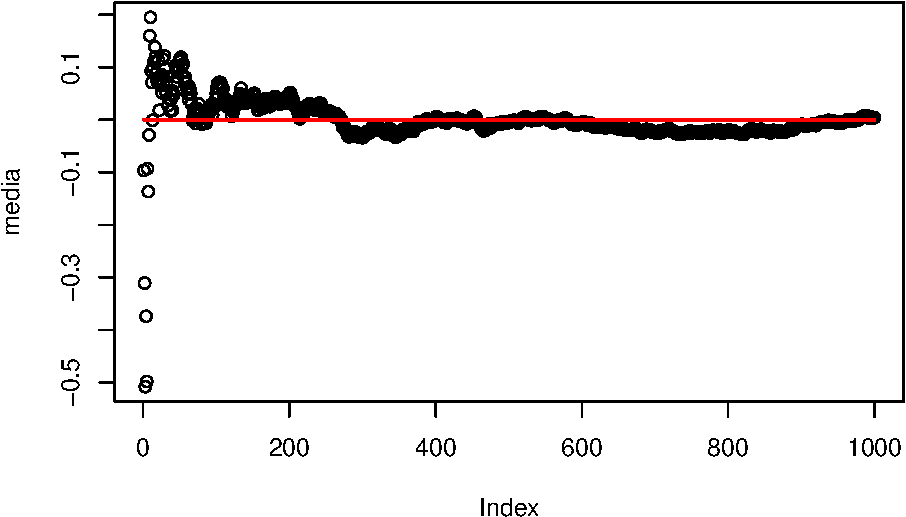
\includegraphics{Bookdown_files/figure-latex/unnamed-chunk-38-1.pdf}

Esse é um exemplo básico, mas a ideia é mais poderosa: e se tivermos um
momento da forma \(E(xu)=0\), onde x e u são variáveis aleatórias
univariadas?\footnote{Isso é familiar?} Se a lei dos grandes números é
verdadeira, \(\widehat{E(xu)} = \sum_i x_i u_i\) deve convergir para
zero. Vamos testar seguindo a mesma ideia acima. A única diferença é que
a nossa média vai ter que ser calculada sem a função padrão
\texttt{mean}:

\begin{Shaded}
\begin{Highlighting}[]
\NormalTok{amostra.}\DecValTok{1}\NormalTok{ <-}\StringTok{ }\KeywordTok{rnorm}\NormalTok{(}\DecValTok{1000}\NormalTok{)}
\NormalTok{amostra.}\DecValTok{2}\NormalTok{ <-}\StringTok{ }\KeywordTok{rnorm}\NormalTok{(}\DecValTok{1000}\NormalTok{)}

\NormalTok{prod <-}\StringTok{ }\NormalTok{amostra.}\DecValTok{1}\OperatorTok{*}\NormalTok{amostra.}\DecValTok{2}

\NormalTok{momento <-}\StringTok{ }\KeywordTok{rep}\NormalTok{(}\DecValTok{0}\NormalTok{,}\DecValTok{1000}\NormalTok{)}

\ControlFlowTok{for}\NormalTok{(i }\ControlFlowTok{in} \DecValTok{1}\OperatorTok{:}\DecValTok{1000}\NormalTok{)\{}
\NormalTok{  momento[i] <-}\StringTok{ }\DecValTok{1}\OperatorTok{/}\NormalTok{i}\OperatorTok{*}\KeywordTok{sum}\NormalTok{(prod[}\DecValTok{1}\OperatorTok{:}\NormalTok{i])}
\NormalTok{\}}

\KeywordTok{plot}\NormalTok{(momento)}
\KeywordTok{lines}\NormalTok{(}\DecValTok{1}\OperatorTok{:}\DecValTok{1000}\NormalTok{,}\KeywordTok{rep}\NormalTok{(}\DecValTok{0}\NormalTok{,}\DecValTok{1000}\NormalTok{), }\DataTypeTok{col=} \DecValTok{2}\NormalTok{, }\DataTypeTok{lwd =} \DecValTok{2}\NormalTok{)}
\end{Highlighting}
\end{Shaded}

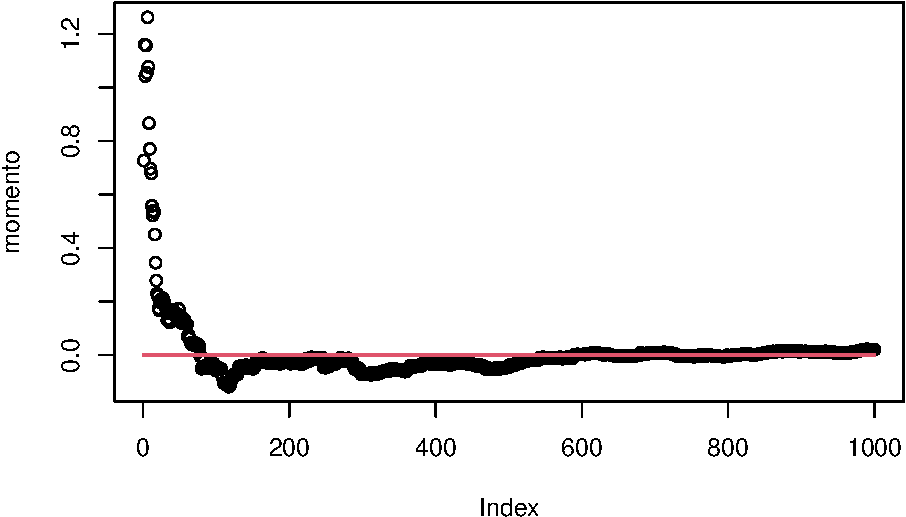
\includegraphics{Bookdown_files/figure-latex/unnamed-chunk-39-1.pdf}

\section{Mínimos Quadrados
Ordinários}\label{minimos-quadrados-ordinarios-1}

Dificuldade

Intermediário

Capítulos necessários

1, 6, 5 (Só a seção de if)

Eu uso matrizes extensivamente nesse exemplo!

O estimador de MQO é o estimador mais fundamental da econometria. Existe
mais de uma maneira de derivar ele: podemos ver como um problema de
minimização, como fizemos no capítulo 8; aqui, vamos derivar ele a
partir da condição de momento \(E(xu) = 0\) para todo x, e onde \(u\)
representa o erro. Veja que se fizermos uma matriz \(X\), que tem em
cada linha uma observação e em cada coluna uma variável, e
\(\mathbf{u}\) o vetor de erros \(n \times{} 1\), \(\mathbf{y}\), o
vetor da variável dependente também \(n \times{} 1\), então a condição
de momento se torna \(E(X^{'}\mathbf{u})=0\). Se expandirmos isso,
usando o fato que \(\mathbf{u} = \mathbf{y}-X\beta\). Então:

\[E(X^{'}\mathbf{u})=E(X^{'}(\mathbf{y}-X\beta))=E(X^{'}\mathbf{y})-E(X^{'}X)\beta = 0 \therefore E(X^{'}\mathbf{y})=E(X^{'}X)\beta \therefore \beta_{OLS} = E(X^{'}X)^{-1}E(X^{'}\mathbf{y})\]
Vamos implementar ele no R. Vamos criar uma função que pega a matriz
\(X\) e o vetor y e faz a conta para obter o MQO. Precisamos de:

\begin{itemize}
\tightlist
\item
  \texttt{\%*\%}, que multiplica duas matrizes, ou um vetor e uma matriz
\item
  \texttt{solve}que inverte a matriz
\item
  \texttt{t}que transpõe a matriz
\end{itemize}

\begin{Shaded}
\begin{Highlighting}[]
\NormalTok{mqo <-}\StringTok{ }\ControlFlowTok{function}\NormalTok{(x,y)\{}
\NormalTok{  bloco_}\DecValTok{1}\NormalTok{ <-}\StringTok{ }\KeywordTok{t}\NormalTok{(x)}\OperatorTok\NormalTok{x}
\NormalTok{  bloco_}\DecValTok{2}\NormalTok{ <-}\StringTok{ }\KeywordTok{t}\NormalTok{(x)}\OperatorTok\NormalTok{y}
  \KeywordTok{return}\NormalTok{(}\KeywordTok{solve}\NormalTok{(bloco_}\DecValTok{1}\NormalTok{)}\OperatorTok\NormalTok{bloco_}\DecValTok{2}\NormalTok{)}
\NormalTok{\}}
\end{Highlighting}
\end{Shaded}

Com uma meia dúzia de manipulações (trocando o \(y\) do \(\beta_{OLS}\)
por \(u\) e fazendo \(\beta \beta^{'}\)), obtemos a expressão para a
variância do estimador de OLS:

\[Var(\beta_{OLS}) = (X^{'}X)^{-1}X^{'}DX(X^{'}X)^{-1}\]

Onde \(D\) é uma matriz diagonal cuja as entradas na diagonal são os
elementos da diagonal de \(uu^{'}\)\footnote{Veja que fora da diagonal
  temos apenas zeros: isso faz sentido no caso iid, onde não esperamos
  correlação entre os erros}. Então, para obtermos a variância do OLS,
precisamos calcular primeiro o resíduo. Vamos criar duas funções: uma
para calcular os resíduos, e outra que calcula a variância do
\(\beta_{OLS}\). A função que calcula a variância vai chamar a função
que calcula os resíduos. Veja que podemos fazer essas funções de várias
maneiras: a função que calcula o resíduo pode recber só o X e y e chamar
a função \texttt{mqo} para fazer a conta do coeficiente; ou a função
pode receber X,y \emph{e} o coeficiente para calcular o resíduo. Eu vou
escolher o segundo caminho:

\begin{Shaded}
\begin{Highlighting}[]
\NormalTok{residuo <-}\StringTok{ }\ControlFlowTok{function}\NormalTok{(x,y,cofs)\{}
\NormalTok{  u <-}\StringTok{ }\NormalTok{y }\OperatorTok{-}\StringTok{ }\NormalTok{x}\OperatorTok\NormalTok{cofs}
  \KeywordTok{return}\NormalTok{(u)}
\NormalTok{\}}

\NormalTok{variancia_mqo <-}\StringTok{ }\ControlFlowTok{function}\NormalTok{(x,y)\{}
\NormalTok{  cof <-}\StringTok{ }\KeywordTok{mqo}\NormalTok{(x,y)}
\NormalTok{  res <-}\StringTok{ }\KeywordTok{residuo}\NormalTok{(x,y,cof)}
\NormalTok{  bloco_}\DecValTok{1}\NormalTok{ <-}\StringTok{ }\KeywordTok{solve}\NormalTok{(}\KeywordTok{t}\NormalTok{(x)}\OperatorTok\NormalTok{x)}
\NormalTok{  D <-}\StringTok{ }\KeywordTok{matrix}\NormalTok{(}\DecValTok{0}\NormalTok{,}\DataTypeTok{ncol =} \KeywordTok{nrow}\NormalTok{(x),}\DataTypeTok{nrow=}\KeywordTok{nrow}\NormalTok{(x))}
  \KeywordTok{diag}\NormalTok{(D) <-}\StringTok{ }\KeywordTok{diag}\NormalTok{(res}\OperatorTok\KeywordTok{t}\NormalTok{(res)) }\CommentTok{#diag acessa os elmentos da diagonal da matriz: logo, eu estou contando para o R que os elementos da diagonal de D são os elmentos da diagonal de res*res'}
\NormalTok{  resposta <-}\StringTok{ }\NormalTok{bloco_}\DecValTok{1}\OperatorTok\KeywordTok{t}\NormalTok{(x)}\OperatorTok\NormalTok{D}\OperatorTok\NormalTok{x}\OperatorTok\KeywordTok{t}\NormalTok{(bloco_}\DecValTok{1}\NormalTok{)}
  \KeywordTok{return}\NormalTok{(resposta)}
\NormalTok{\}}
\end{Highlighting}
\end{Shaded}

Veja que a função \texttt{variancia\_mqo}recebe só \(X\) e y e todo o
resto das contas são feitos por funções que criamos originalmente: o
coeficiente é calculado pela função \texttt{mqo}, que passa isso para a
função \texttt{residuo}, que por sua vez passa o resultado para obtermos
a variância do estimador.

Vamos construir uma função final que devolve os coeficientes e o erro
padrão. Mais ainda, eu vou adicionar uma mopção que adiciona um
intercepto (as funções acima não fazem isso!). Para isso, observe que um
intercepto é somente colar uma coluna de 1s na matriz X. Então, na
função \texttt{regressao}, eu vou adicionar uma opção
\texttt{intercepto}, que vai ser um booleano (verdadeiro ou falso). Se
for verdadeiro, eu adiciono uma coluna de 1s. Se você apostou que eu vou
fazer isso usando um \texttt{if}, parabéns: é exatamente o que eu vou
fazer. Para deixar a coisa mais completa, a função vai ter como padrão
adicionar o intercepto:

\begin{Shaded}
\begin{Highlighting}[]
\NormalTok{regressao <-}\StringTok{ }\ControlFlowTok{function}\NormalTok{(x,y,}\DataTypeTok{intercepto =}\NormalTok{ T)\{}
  \ControlFlowTok{if}\NormalTok{(intercepto }\OperatorTok{==}\StringTok{ }\NormalTok{T)\{}
\NormalTok{    x <-}\StringTok{ }\KeywordTok{cbind}\NormalTok{(}\DecValTok{1}\NormalTok{,x) }\CommentTok{#Veja o comentário abaixo}
\NormalTok{  \} }\CommentTok{# como o caso else não faz nada, eu posso simplesmente não colocar nada no else}
\NormalTok{  coefs <-}\StringTok{ }\KeywordTok{mqo}\NormalTok{(x,y)}
\NormalTok{  vars <-}\StringTok{ }\KeywordTok{diag}\NormalTok{(}\KeywordTok{variancia_mqo}\NormalTok{(x,y)) }\CommentTok{#Diag extrai a diagonal da matriz de variância do coeficiente - e é isso que nos interessa}
  \KeywordTok{return}\NormalTok{(}\KeywordTok{cbind}\NormalTok{(coefs,}\KeywordTok{sqrt}\NormalTok{(vars)))}
\NormalTok{\}}
\end{Highlighting}
\end{Shaded}

Veja que ao fazer \texttt{cbind(1,x)}, o R é inteligente o suficiente
para repetir 1 o número de linhas de x, sem termos que nos preocupar em
definir um vetor 1 do mesmo número de linhas que a matriz \(X\).Vamos
testar a nossa função, comparado com o comando padrão do R, \texttt{lm}:

\begin{Shaded}
\begin{Highlighting}[]
\NormalTok{X <-}\StringTok{ }\KeywordTok{matrix}\NormalTok{(}\KeywordTok{rnorm}\NormalTok{(}\DecValTok{500}\NormalTok{),}\DataTypeTok{ncol =} \DecValTok{5}\NormalTok{)}
\NormalTok{y <-}\StringTok{ }\NormalTok{X}\OperatorTok\KeywordTok{c}\NormalTok{(}\DecValTok{1}\NormalTok{,}\OperatorTok{-}\DecValTok{1}\NormalTok{,}\DecValTok{2}\NormalTok{,}\OperatorTok{-}\DecValTok{2}\NormalTok{,}\FloatTok{0.5}\NormalTok{) }\OperatorTok{+}\StringTok{ }\KeywordTok{rnorm}\NormalTok{(}\DecValTok{100}\NormalTok{)}

\KeywordTok{regressao}\NormalTok{(X,y)}
\end{Highlighting}
\end{Shaded}

\begin{verbatim}
##             [,1]      [,2]
## [1,] -0.08762789 0.1051556
## [2,]  1.02427340 0.1109157
## [3,] -0.73255790 0.1175446
## [4,]  1.86708375 0.1238537
## [5,] -1.92379372 0.1133978
## [6,]  0.59176754 0.1074243
\end{verbatim}

\begin{Shaded}
\begin{Highlighting}[]
\KeywordTok{summary}\NormalTok{(}\KeywordTok{lm}\NormalTok{(y }\OperatorTok{~}\StringTok{ }\NormalTok{X))}
\end{Highlighting}
\end{Shaded}

\begin{verbatim}
## 
## Call:
## lm(formula = y ~ X)
## 
## Residuals:
##     Min      1Q  Median      3Q     Max 
## -2.3389 -0.6190 -0.0333  0.5789  3.1919 
## 
## Coefficients:
##             Estimate Std. Error t value Pr(>|t|)    
## (Intercept) -0.08763    0.11101  -0.789    0.432    
## X1           1.02427    0.10243   9.999  < 2e-16 ***
## X2          -0.73256    0.11738  -6.241 1.24e-08 ***
## X3           1.86708    0.13121  14.230  < 2e-16 ***
## X4          -1.92379    0.12272 -15.676  < 2e-16 ***
## X5           0.59177    0.11235   5.267 8.75e-07 ***
## ---
## Signif. codes:  0 '***' 0.001 '**' 0.01 '*' 0.05 '.' 0.1 ' ' 1
## 
## Residual standard error: 1.064 on 94 degrees of freedom
## Multiple R-squared:  0.854,  Adjusted R-squared:  0.8463 
## F-statistic:   110 on 5 and 94 DF,  p-value: < 2.2e-16
\end{verbatim}

Veja que há uma leve diferença entre os erros padrões computados pela
minha função e pelo \texttt{lm}. Isso se deve ao fato do R assumir erros
homocedásticos e a matriz de variância covariância que nós implementamos
não assume isso.

\section{LASSO}\label{lasso}

Dificuldade

Intermediário

Capítulos necessários

8 e 6 (somente para o último passo)

LASSO (Least Absolute Shrinkage and Selection Operator) é uma maneira de
fazer regressão quando temos muitas variáveis e queremos selecionar só
as que são relevantes - potencialmente, podemos ter mais variáveis que
observações! Formalmente, o LASSO resolve:

\[\beta_{LASSO} = \text{argmin}_\beta \sum_i (y_i - x_i\beta) \text{ sujeito a } \sum_k |\beta_k| < c\]
Onde k indexa as variáveis do problema. No fundo, estamos resolvendo o
problema de minimização usual de mínimos quadrados, com uma restrição: a
soma do valor \emph{absoluto} dos coeficientes não pode passar de um
valor \(c\), que tem que ser determinado\footnote{Não vou entrar nessa
  discussão, mas o que as implementações fazem, em geral, é colocar
  vários valores de \(c\), desde baixos o bastante para que nenhuma
  variável ser incluída até um valor alto suficiente que todas são
  incluídas. Como escolher qual desses \(c\) usar não é óbvio.}. Veja
que, por incrível que pareça, o fato de usarmos o valor absoluto é
bastante importante: usar uma restrição com a soma dos quadrados reduz
os coeficientes, mas não joga nenhum deles para zero. Uma explicação
bastante intuitiva sobre o porque usar o valor absoluto e mais sobre o
LASSO em geral, pode ser encontrada no excelente \emph{Statistical
Learning with Sparsity}, de Trevor Hastie, Robert Tibshirani e Martin
Wainwright (que pode ser encontrado
\href{https://web.stanford.edu/~hastie/StatLearnSparsity_files/SLS_corrected_1.4.16.pdf}{aqui})

Vamos implementar o LASSO usando o CVXR. Vamos criar um conjunto de de
variáveis \(X\), com 100 observações e 50 variáveis, e definir um \(y\)
que depende de alguma dessas variáveis (as 10 primeiras, talvez. Mas não
muito mais que isso!). Escolha os coeficientes que quiser, mas tente
manter os coeficientes longe de zero. Eu escolherei, preguisosamente, 1
para todas as variáveis relevantes. Adicione algum erro no y, exatamente
imitando o problema usual de uma regressão. O passo seguinte é escrever
o programa do CVXR e mandar ele resolver o nosso problema:

\begin{Shaded}
\begin{Highlighting}[]
\NormalTok{X <-}\StringTok{ }\KeywordTok{matrix}\NormalTok{(}\KeywordTok{rnorm}\NormalTok{(}\DecValTok{5000}\NormalTok{),}\DataTypeTok{ncol =} \DecValTok{50}\NormalTok{)}
\NormalTok{beta <-}\StringTok{ }\KeywordTok{c}\NormalTok{(}\KeywordTok{rep}\NormalTok{(}\DecValTok{1}\NormalTok{,}\DecValTok{10}\NormalTok{),}\KeywordTok{rep}\NormalTok{(}\DecValTok{0}\NormalTok{,}\DecValTok{40}\NormalTok{))}
\NormalTok{y <-}\StringTok{ }\NormalTok{X}\OperatorTok\NormalTok{beta }\OperatorTok{+}\StringTok{ }\KeywordTok{rnorm}\NormalTok{(}\DecValTok{100}\NormalTok{)}

\KeywordTok{library}\NormalTok{(CVXR)}

\NormalTok{c <-}\StringTok{ }\DecValTok{10} \CommentTok{#esse é o valor que vai limitar a soma do valor dos coeficientes. Eu escolhi o valor exato que é a soma dos meus coeficientes, mas você pode (e deve) brincar com isso aqui}

\NormalTok{beta_hat <-}\StringTok{ }\KeywordTok{Variable}\NormalTok{(}\DecValTok{50}\NormalTok{)}
\NormalTok{obj <-}\StringTok{ }\KeywordTok{Minimize}\NormalTok{(}\KeywordTok{sum}\NormalTok{((y}\OperatorTok{-}\NormalTok{X}\OperatorTok\NormalTok{beta_hat)}\OperatorTok{^}\DecValTok{2}\NormalTok{)) }\CommentTok{#essa é a função objetivo}
\NormalTok{cons <-}\StringTok{ }\KeywordTok{sum}\NormalTok{(}\KeywordTok{abs}\NormalTok{(beta_hat)) }\OperatorTok{<}\StringTok{ }\NormalTok{c}
\NormalTok{prob <-}\StringTok{ }\KeywordTok{Problem}\NormalTok{(obj,}\DataTypeTok{constraints =} \KeywordTok{list}\NormalTok{(cons))}
\NormalTok{soluc <-}\StringTok{ }\KeywordTok{solve}\NormalTok{(prob)}
\NormalTok{est <-}\StringTok{ }\NormalTok{soluc}\OperatorTok{$}\KeywordTok{getValue}\NormalTok{(beta_hat) }\CommentTok{#para extrair os betas estimados}
\NormalTok{est[est}\OperatorTok{<}\FloatTok{1e-9}\NormalTok{] <-}\StringTok{ }\DecValTok{0} \CommentTok{#Veja o comentário abaixo}
\NormalTok{est}
\end{Highlighting}
\end{Shaded}

\begin{verbatim}
##              [,1]
##  [1,] 0.952064880
##  [2,] 0.927405698
##  [3,] 0.623051947
##  [4,] 0.833205454
##  [5,] 0.995166633
##  [6,] 0.914978956
##  [7,] 0.845659633
##  [8,] 0.795418403
##  [9,] 0.839713717
## [10,] 0.885603800
## [11,] 0.067397795
## [12,] 0.000000000
## [13,] 0.000000000
## [14,] 0.048155418
## [15,] 0.000000000
## [16,] 0.000000000
## [17,] 0.000000000
## [18,] 0.000000000
## [19,] 0.206185854
## [20,] 0.000000000
## [21,] 0.000000000
## [22,] 0.035731386
## [23,] 0.000000000
## [24,] 0.000000000
## [25,] 0.000000000
## [26,] 0.129196128
## [27,] 0.014904346
## [28,] 0.000000000
## [29,] 0.017190332
## [30,] 0.000000000
## [31,] 0.000000000
## [32,] 0.090893621
## [33,] 0.000000000
## [34,] 0.126430996
## [35,] 0.015774388
## [36,] 0.029822479
## [37,] 0.000000000
## [38,] 0.025583701
## [39,] 0.000000000
## [40,] 0.016902530
## [41,] 0.000000000
## [42,] 0.000000000
## [43,] 0.197721479
## [44,] 0.000000000
## [45,] 0.102971074
## [46,] 0.000000000
## [47,] 0.003457017
## [48,] 0.000000000
## [49,] 0.000000000
## [50,] 0.000000000
\end{verbatim}

Veja que, além do CVXR, eu adicionei um
\texttt{est{[}est\textless{}1e-9{]}\ \textless{}-\ 0}. Como já dito no
Capítulo 8, estimativas númericas nunca vão chegar exatamente em zero.
Então, para deixar o \emph{output} mais legível, eu estou estabelecendo
que qualquer valor abaixo de \(10^{-9}\) é zero. Veja que \(10^{-9}\) é
arbitrário e as implementações de verdade usam padrões estabelecidos.

Voltando ao LASSO: veja que o algoritmo faz um bom trabalho, zerando
vários coeficientes. Ele não zera todos os coeficientes das variáveis
que não deveriam ser incluídas, mas em compensação não zera nenhum
coeficiente das variáveis que deveriam ser incluídas. Trocando em
miúdos: ele dá falsos positivos, mas não falsos negativos. Isso é
verdade, em geral.

Obviamente, o trabalho fica bem mais limpo se escrevermos uma função que
faz tudo isso para quaisquer X,y e c escolhidos. Aproveite o código que
já escrevemos e escreva uma função que faça isso para qualquer X,y e c.
Não esqueça que você vai ter que alterar o tamanho do \texttt{beta\_hat}
(Dica: veja o comando \texttt{ncol}).

\begin{Shaded}
\begin{Highlighting}[]
\NormalTok{lasso <-}\StringTok{ }\ControlFlowTok{function}\NormalTok{(X,y,c)\{}
\NormalTok{  beta_hat <-}\StringTok{ }\KeywordTok{Variable}\NormalTok{(}\KeywordTok{ncol}\NormalTok{(X))}
\NormalTok{  obj <-}\StringTok{ }\KeywordTok{Minimize}\NormalTok{(}\KeywordTok{sum}\NormalTok{((y}\OperatorTok{-}\NormalTok{X}\OperatorTok\NormalTok{beta_hat)}\OperatorTok{^}\DecValTok{2}\NormalTok{)) }\CommentTok{#essa é a função objetivo}
\NormalTok{  cons <-}\StringTok{ }\KeywordTok{sum}\NormalTok{(}\KeywordTok{abs}\NormalTok{(beta_hat)) }\OperatorTok{<}\StringTok{ }\NormalTok{c}
\NormalTok{  prob <-}\StringTok{ }\KeywordTok{Problem}\NormalTok{(obj,}\DataTypeTok{constraints =} \KeywordTok{list}\NormalTok{(cons))}
\NormalTok{  soluc <-}\StringTok{ }\KeywordTok{solve}\NormalTok{(prob)}
\NormalTok{  est <-}\StringTok{ }\NormalTok{soluc}\OperatorTok{$}\KeywordTok{getValue}\NormalTok{(beta_hat) }\CommentTok{#para extrair os betas estimados}
\NormalTok{  est[est}\OperatorTok{<}\FloatTok{1e-9}\NormalTok{] <-}\StringTok{ }\DecValTok{0} \CommentTok{#Veja o comentário abaixo}
  \KeywordTok{return}\NormalTok{(est)}
\NormalTok{\}}
\end{Highlighting}
\end{Shaded}

Veja que eu fui tão preguiçoso ao escrever a função que nem mesmo os
comentários mudaram!

Em situações em que você queira usar o LASSO, o pacote \textbf{glmnet}
faz o LASSO até mesmo para modelos Probit e Logit, e é infinitamente
superior a implementação acima.

\chapter{Referências}\label{referencias}

Todas as referências a seguir são em inglês. Isso reflete justamente a
limitação da literatura em português sobre R e economia - o exato motivo
da confecção deste manual.

\section{R}\label{r}

Dois livros foram essenciais para este autor aprender a usar o R: o
\emph{R Book}, de Michael J. Crawley e o \emph{Applied Econometrics with
R}, de Christian Kleiber e Achim Zeileis. O primeiro é extremamente
geral e cobre de tudo, explicando muito dos tópicos tratados aqui
superficialmente com muito mais detalhes. O segundo tem um título auto
explicativo.

\section{Tidyverse}\label{tidyverse}

Uma omissão notável desse manual são os pacotes do \emph{Tidyverse},
especialmente o Dplyr e o ggplot, que são muito usados para limpar dados
e fazer gráficos, respectivamente. O autor desses pacotes, Hadley
Wickham, tem um excelente livro sobre como fazer ciência de dados no R,
chamado \emph{R for Data Science}, e que o próprio disponibiliza
\href{http://r4ds.had.co.nz/}{aqui}. O
\href{https://www.tidyverse.org/}{site do Tidyverse} também traz
excelentes recursos de como usar esses pacotes.

\section{LaTeX}\label{latex}

Um dos melhores recursos para aprender LaTeX é o livro da wikipedia
sobre a linguagem, disponível
\href{https://en.wikibooks.org/wiki/LaTeX}{aqui}. Felizmente, não é
sequer necessário instalar o LaTeX no computador, já que existem
serviços online que fornecem armazenamento e um editor de LaTeX online.
Os dois mais famosos são o \href{https://www.overleaf.com/}{overleaf} e
o \href{https://pt.sharelatex.com/}{sharelatex}.


\end{document}
